%%%%%%%%%%%%%%%%%%%%%%%%%%%%%%%%%%%%%%%%%
% Masters/Doctoral Thesis 
% LaTeX Template
% Version 1.43 (17/5/14)
%
% This template has been downloaded from:
% http://www.LaTeXTemplates.com
%
% Original authors:
% Steven Gunn 
% http://users.ecs.soton.ac.uk/srg/softwaretools/document/templates/
% and
% Sunil Patel
% http://www.sunilpatel.co.uk/thesis-template/
%
% License:
% CC BY-NC-SA 3.0 (http://creativecommons.org/licenses/by-nc-sa/3.0/)
%
% Note:
% Make sure to edit document variables in the Thesis.cls file
%
%%%%%%%%%%%%%%%%%%%%%%%%%%%%%%%%%%%%%%%%%

%----------------------------------------------------------------------------------------
%	PACKAGES AND OTHER DOCUMENT CONFIGURATIONS
%----------------------------------------------------------------------------------------

\documentclass[11pt, oneside]{Thesis} % The default font size and one-sided printing (no margin offsets)

\graphicspath{{Pictures/}} % Specifies the directory where pictures are stored

\usepackage[square, numbers, comma, sort&compress]{natbib} % Use the natbib reference package - read up on this to edit the reference style; if you want text (e.g. Smith et al., 2012) for the in-text references (instead of numbers), remove 'numbers' 
\hypersetup{urlcolor=blue, colorlinks=true} % Colors hyperlinks in blue - change to black if annoying
\title{\ttitle} % Defines the thesis title - don't touch this

\begin{document}

\frontmatter % Use roman page numbering style (i, ii, iii, iv...) for the pre-content pages

\setstretch{1.3} % Line spacing of 1.3

% Define the page headers using the FancyHdr package and set up for one-sided printing
\fancyhead{} % Clears all page headers and footers
\rhead{\thepage} % Sets the right side header to show the page number
\lhead{} % Clears the left side page header

\pagestyle{fancy} % Finally, use the "fancy" page style to implement the FancyHdr headers

\newcommand{\HRule}{\rule{\linewidth}{0.5mm}} % New command to make the lines in the title page

% PDF meta-data
\hypersetup{pdftitle={\ttitle}}
\hypersetup{pdfsubject=\subjectname}
\hypersetup{pdfauthor=\authornames}
\hypersetup{pdfkeywords=\keywordnames}

%----------------------------------------------------------------------------------------
%	TITLE PAGE
%----------------------------------------------------------------------------------------

\begin{titlepage}
\begin{center}

\textsc{\LARGE \univname}\\[1.5cm] % University name
%\textsc{\Large Doctoral Thesis}\\[0.5cm] % Thesis type

\HRule \\[0.4cm] % Horizontal line
{\huge \bfseries \ttitle}\\[0.4cm] % Thesis title
\HRule \\[1.5cm] % Horizontal line
 
\begin{minipage}{0.4\textwidth}
\begin{flushleft} \large
\emph{Author:}\\
\href{http://www.johnsmith.com}{\authornames} % Author name - remove the \href bracket to remove the link
\end{flushleft}
\end{minipage}
\begin{minipage}{0.4\textwidth}
\begin{flushright} \large
\emph{Supervisor:} \\
\href{http://www.jamessmith.com}{\supname} % Supervisor name - remove the \href bracket to remove the link  
\end{flushright}
\end{minipage}\\[3cm]
 
% \large \textit{A thesis submitted in fulfilment of the requirements\\ for the degree of \degreename}\\[0.3cm] % University requirement text
% \textit{in the}\\[0.4cm]
\deptname\\[2cm] % Research group name and department name
 
{\large \today}\\[4cm] % Date
%\includegraphics{Logo} % University/department logo - uncomment to place it
 
\vfill
\end{center}

\end{titlepage}


%----------------------------------------------------------------------------------------
%	ABSTRACT PAGE
%----------------------------------------------------------------------------------------

\addtotoc{Abstract} % Add the "Abstract" page entry to the Contents

\abstract{\addtocontents{toc}{\vspace{1em}} % Add a gap in the Contents, for aesthetics

This thesis proposes a multicore architecture that
allows fault tolerant cores to distribute critical tasks to less
reliable cores. The fault tolerant core makes use of a distributed fingerprinting system to monitor other cores and a
centralized hardware comparator that gathers and compares
fingerprints. Fingerprinting represents an additional hardware
cost but provides significantly lower detection latencies compared
to software voting on the fault tolerant core. Fingerprinting
requires no changes to the microarchitecture of the processor and
is therefore easier to integrate into preexisting designs compared
to single core hardening techniques. We have developed an
FPGA prototype using Altera Nios II cores that successfully
fingerprints parallel thread executions on arbitrary pairs of cores.
We have also developed a virtual debugging platform for future hardware and software development using OVP processor models and the Imperas M*SDK multicore simulation and debugging tool chain.
The fingerprinting unit represents 15\% of the core resources in
combinational logic and 3\% of memory bits while the comparator
adds 6\% cost to the system and consumes less than 5\% of
memory.
}

\clearpage % Start a new page



%----------------------------------------------------------------------------------------
%	LIST OF CONTENTS/FIGURES/TABLES PAGES
%----------------------------------------------------------------------------------------

\pagestyle{fancy} % The page style headers have been "empty" all this time, now use the "fancy" headers as defined before to bring them back

\lhead{\emph{Contents}} % Set the left side page header to "Contents"
\tableofcontents % Write out the Table of Contents

\lhead{\emph{List of Figures}} % Set the left side page header to "List of Figures"
\listoffigures % Write out the List of Figures

\lhead{\emph{List of Tables}} % Set the left side page header to "List of Tables"
\listoftables % Write out the List of Tables

\lhead{\emph{List of Listings}} % Set the left side page header to "List of Tables"
\lstlistoflistings % Write out the List of Tables

%----------------------------------------------------------------------------------------
%	ABBREVIATIONS
%----------------------------------------------------------------------------------------

\clearpage % Start a new page

\setstretch{1.5} % Set the line spacing to 1.5, this makes the following tables easier to read

\lhead{\emph{Abbreviations}} % Set the left side page header to "Abbreviations"
\listofsymbols{ll} % Include a list of Abbreviations (a table of two columns)
{
\textbf{DCC} & \textbf{D}ynamic \textbf{C}ore \textbf{C}oupling \\
\textbf{DMR} & \textbf{D}ual \textbf{M}odular \textbf{R}edundancy \\
\textbf{ES} & \textbf{E}execution \textbf{S}tream \\
\textbf{FID} & \textbf{F}ingerprint \textbf{ID}entification \\
\textbf{FP} & \textbf{F}inger\textbf{P}rint \\
\textbf{FTC} & \textbf{F}ault \textbf{T}olerant \textbf{C}ore \\
\textbf{ODR} & \textbf{O}n \textbf{D}emand \textbf{R}edundancy \\
\textbf{RTOS} & \textbf{R}eal \textbf{T}ime \textbf{O}perating \textbf{S}ystem \\
\textbf{SoR} & \textbf{S}phere of \textbf{R}eplication \\

%\textbf{Acronym} & \textbf{W}hat (it) \textbf{S}tands \textbf{F}or \\
}

%----------------------------------------------------------------------------------------
%	THESIS CONTENT - CHAPTERS
%----------------------------------------------------------------------------------------

\mainmatter % Begin numeric (1,2,3...) page numbering

\pagestyle{fancy} % Return the page headers back to the "fancy" style

\definecolor{mygreen}{rgb}{0,0.6,0}
\definecolor{mygray}{rgb}{0.5,0.5,0.5}
\definecolor{mymauve}{rgb}{0.58,0,0.82}

\lstset{numbers=left,
        commentstyle=\color{mygreen},
        keywordstyle=\color{blue},       % keyword style
        language=C,                 % the language of
        stringstyle=\color{mymauve}
}
% Include the chapters of the thesis as separate files from the Chapters folder
% Uncomment the lines as you write the chapters

 % Chapter 1

\chapter{Architecture Overview} % Main chapter title

\label{Chapter1} % For referencing the chapter elsewhere, use \ref{Chapter1} 

\lhead{Chapter 1. \emph{Architecture Overview}} % This is for the header on each page - perhaps a shortened title

%----------------------------------------------------------------------------------------

\section{Introduction}

In safety critical systems it is sometimes necessary to use redundancy to ensure that the output from a processor is valid. The most common method of building a system with redundancy today is called lockstep execution or dual modular redundancy (DMR). In DMR, the entire processor core is replicated and outputs from store instructions are kept in a buffer until it can be verified that the data and addresses of both cores match. There are several disadvantages related to the scalability of lockstep execution given in \cite{lafrieda2007utilizing}:
\begin{itemize}
\item The temperature and energy requirements for lockstep cores are very high because "DMR pairs running code with similar power/thermal characteristics are necessarily placed next to each other on the die."
\item It is not possible for the cores to execute independently. This also means that if there is a permanent fault in one core, then neither core can be used.
\item The performance of the cores must be very precise and kept synchronized at the level of individual instructions (although there is often a small delay between thread executions on the order of tens of instructions).
\item Core pairs with different frequency or leakage characteristics are bounded by the performance of the slower core.
\item The cummulative effect of the previous items make it difficult to envision a practical and scalable multicore solution to redundancy that relies mainly on lockstep for all resources.
\end{itemize}
The advantages of lockstep include:
\begin{itemize}
\item The detection of errors requires no software intervention or supervision.
\item Code requires no special modifications to be ported onto a lockstep architecture.
\item There is no significant impact on the predictability or execution time of code on the DMR pair compared to a single core.
\item Error correction by voting can be accomplished by increasing the amount of redundancy.
\end{itemize}

Some sections of this thesis (mainly Chapter 1 and Chapter 5) are also being submitted as part of a conference paper.

\subsection{Scalable alternatives to lockstep execution}

\textit{Fingerprinting} is one of many possible alternatives or evolutions to lockstep and DMR. The main insight behind fingerprinting is that it is possible to compare hashes or fingerprints (FPs) calculated based on the activity of a processor core (execution stream or ES) rather than directly comparing the ES itself. The ES in its simplest form consists of store addresses and data however it can also include load addresses and changes to the register file. 

Fingerprinting has been an important component of several proposed architectural features over the last decade that demonstrated promising preliminary results in simulation. These features attempt to resolve the limitations of lockstep DMR that make it difficult to scale with the number of cores of an MPSoC. 

Another feature of commonly predicted in future distributed embedded systems is a \emph{mixed criticality} workload. Mixed criticality is "the integration of applications of different criticality (safety, security, real-time and non-real time) in a single embedded
system" \cite{perez2013safety}. Besides possible high level advantages that can emerge from improved allocation of resources, integrating distributed systems onto a single chip can improve the amount of wiring in a system dramatically. It is claimed in \cite{swingler2000degradation} that 30-60\% of automotive system failures are attributable to interconnect failures. 

System features related to the improvement of resource allocation and application scheduling are:
\begin{itemize}
\item \textit{On-Demand Redundancy:} One natural target for increasing efficiency is to allow cores to be able to execute independent tasks or applications in parallel when redundancy is not required. It is wasteful to run an application that does not require redundancy on a pair of cores in lockstep. Ideally, applications could monitor critical tasks and detect errors with redundancy services provided by the system while allowing less critical tasks to run independently and concurrently on the two cores.
\item \textit{Dynamic Core Coupling (DCC):} Consider attempting to derive a static schedule for several applications on an MPSoC with six or eight cores where redundancy services are available on-demand. One possibility is to provide redundancy services in hardware by allowing three pairs of cores to execute in lockstep. Again, intuitively, an optimal solution is more likely to be found if \textit{any} two cores can be paired in lockstep and if these pairings can be adjusted at runtime. Previous simulation work on DCC has shown much better schedules can be derived when this is the case.
\end{itemize}

In order to provide the flexibility of DCC a system must be able to monitor the ES, establish a sphere of replication (SoR) by which errors are contained and not allowed to contaminate main memory, and provide a mechanism for comparing the ES of different cores independently of interconnect topology. Software and hardware overhead related to the management of monitoring resources must be kept to a minimum. As previous authors have noted, hardware monitoring of the ES is preferable but the amount of information required to compare the ES of different cores must be reduced. Fingerprinting is an important component to designing a system with these characteristics. 

The integration of partitioning and resource allocation through hypervisors and health-monitoring services such as those proposed for the monitor core in the ACROSS platform provide an interesting starting point for the development of a comprehensive fault tolerance strategy aimed at multicore platforms. While we are not yet able to either duplicate or integrate a hypervisor, we can allow them to inform our design choices.

\begin{figure}[h]
\centering
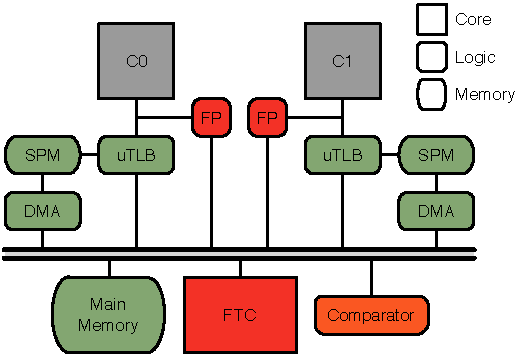
\includegraphics[scale=1.5]{Figures/architecture}
\caption{System view of hardware platform.}
\label{f:arch}
\end{figure}

We propose a novel system implementing heterogeneous reliability, presented in Figure \ref{f:arch}, that provides the necessary hardware functionality to support dynamic core coupling and on-demand redundancy, and broaden the scope of design-space exploration for reliability-constrained cost optimization.
	We have designed the required logic, written simple drivers, and demonstrated the ease with which fingerprinting can be integrated into a traditional RTOS environment.	
	This architecture utilizes:
\begin{itemize}
\item	\emph{Fingerprinting logic} to compress modifications to external state into a single, fixed-width word;
\item	\emph{Scratch-pad memories, $\mu$TLBs, and DMAs} to manage modified state under quarantine until redundancy checking has been performed on corresponding fingerprints;
\item	Scalable \emph{comparison logic} to identify and compare matching fingerprints when their corresponding instructions segments have finished executing; and
\item	A \emph{fault-tolerant core} to execute safety-critical tasks, and coordinate the activity of the above units to safely monitor critical tasks executing on unreliable processors.
\end{itemize}
	The above hardware can be unintrusively integrated with the host processor system, and requires no modification to the processor core or compiler.
	When not needed, redundancy checking may be disabled, freeing resources to perform other tasks independently and therefore improving performance relative to lockstep execution (under which redundancy checking is continually performed)~\cite{Meyer:CASES11}.
	
\section{Related Work}
\subsection{The ACROSS MPSoC}


The ACROSS MPSoC was a joint project of 16 European partners from industry and academia. It is a comprehensive multicore architecture combining time triggered network fabric and up to ten cores to provide reliable and deterministic application execution \cite{el2013across}. A recent expansion of the project has been the automatic design space exploration of a reliable embedded system. Models of the application and platform are used to explore the design space of application to resource mappings that take into account reliability and timing requirements. The system automatically generates application source code and platform configuration files \cite{huang2014framework}. Their analysis of of reliable design space exploration  is independent of a specific method of detecting errors. The performance overhead associated with a fault tolerance mechanism are simply another parameter in the platform model that will inform the search for an optimal allocation of resources. 


%The ACROSS MPSoC is at the center of a large project that aims to demonstrate a highly predictable multicore architecture for safety-critical and general real-time multicore distributed systems. The project has proceeded to using platform modelling to generate distributed application code for the entire system based on performance parameters.The criticality of an application is one such parameter used to determine if a task should be replicated on several cores. However, while the existence of several proposed mechanisms for capturing and comparing the ES are known, there is yet to be a realistic architectural solution that that can be implemented with current technology. This platform is such an architecture and we borrow heavily from the ACROSS project. Many assumptions made about parts of the system that have yet to be implemented are based on results stemming from the ACROSS project.

One key feature of the ACROSS platform is the reservation of certain cores for monitoring the rest of the system \cite{kopetz2007automotive}. One of the special cores is the \textit{diagnostic core} which uses information from local \textit{health monitoring services} belonging to the general purpose cores to detect anomalies. We believe this vision for distributed multicore platforms to be very promising and that fingerprinting can play an important role in monitoring services in such a platform for mixed-criticality applications requiring redundancy. 

Taken from Huang et al. \cite{huang2014framework}:
\begin{quote}
Our approach is based on the following:
\begin{itemize}
\item Platform-independent description of the application including timing and reliability requirements.
\item Fine-grained platform model covering both hardware platform
and system software (HW/SW stack).

\item Multi-criteria design space exploration: mapping and scheduling w.r.t. timing and reliability constraints (consideration of
permanent and transient faults).
\item Automatic insertion of fault-tolerance techniques, including
active redundancy, voting and fault detection to meet userspecified reliability goals.
\item Generation of implementation artifacts such as application C
source code and platform configuration files.
\end{itemize}
\end{quote}

Their work deliberately avoids committing to a specific fault tolerance mechanism: 
\begin{quote}
The configurability enables the user to select candidate FTMs for
the specific application domain and is therefore essential for the
practical applicability of the approach.
\end{quote}

An ideal fault tolerance mechanism for such a system would be easily managed and customized by software, provide a high degree of flexibility and configurability in terms of error detection strength, and rely on dedicated hardware to minimize the performance impact of monitoring the system. It would also be independent of network or bus topology and place minimal restrictions on scheduling strategies (i.e. it would have minimal impact on an optimization solution that assumes zero overhead). Fingerprinting can be easily viewed as a fine-grained \emph{health-monitoring service} used by the monitor to ensure safe operation of critical tasks.

\subsection{The Xtratum Hypervisor}

Another project that represents significant progress on related issues is the Xtratum hypervisor that is designed for hardware paravirtualization (hardware resources are only partially virtualized to minimize performance overhead in real-time systems) of  and safely implementing mixed criticality systems with provable partitioning mechanisms in place. We have currently only implemented enough software architecture to demonstrate how fingerprinting could be built into an RTOS at the lowest level. We rely on projects such as Xtratum as proof of the types of services that could be integrated with these low level functionalities to provide more developed task replication services making for a sort of plug-and-play DCC. 

The main consideration when it comes to mixed criticality systems and industrial certification is given by Perez et al. in \cite{perez2013safety}:
\begin{quote}The integration of applications of different criticality (safety,
security, real-time and non-real time) in a single embedded
system is referred as mixed-criticality system. This integrated
approach can improve scalability, increase reliability reducing
the amount of systems-wires-connectors and reduce the overall
cost-size-weight factor. However, safety certification according
to industrial standards becomes a challenge because sufficient
evidence must be provided to demonstrate that the resulting
system is safe for its purpose. Higher safety integrity functions
must be interference free with respect to lower safety integrity
functions.
\end{quote}

\subsection{Heterogeneous Reliability}
As with many current trends in embedded systems, the problem of heterogeneous reliability has previously been proposed in the high performance domain \cite{hruby2013slower,he2003reliability,ungsunan2009improving}. Bolchini and Miele explicitly introduce the notion of heterogeneous reliability into the problem of model-based design space exploration for embedded systems \cite{bolchini2013reliability}. They map mixed-criticality applications onto platforms with cores of varying degrees of fault tolerance in terms of strength and cost. They observe that systems with heterogeneous reliability mechanisms can generally provide a wider range of options in terms of optimizing resource utilization given a mixed criticality workload.

Reliability aware scheduling is complex even in the static case due to the need for contingency schedules. In the case where cores are only equipped with the capability to detect but not correct errors, it is necessary to have alternative schedules to reallocate resources so that the critical task deadline is not missed. If several concurrent errors are to be supported, then several branches of contingency schedules are required. In \cite{bolchini2013reliability} it is assumed that tasks can be grouped in order to minimize the amount of software voting tasks required. This creates a tradeoff between voting overhead and detection latency. They assume that the voting overhead should be minimized since errors are rare. 

With fingerprinting, the cost of verifying redundant task executions is completely offloaded into hardware and detection latencies are reduced dramatically. This could eliminate the need for task grouping and simplify the job of developing contingency schedules. If a task within a group fails, then this is only known once the final task in the group completes and the entire group must be rescheduled. With fingerprinting, the amount of work that must be re-executed in the case of an error or errors is reduced dramatically since only a single task is corrupted.

\section{Motivating Example: Scheduling}
\label{s:schedulingstudy}

	Recent work has examined automated design space exploration to map applications onto heterogeneous multicore platforms \cite{bolchini2013reliability,huang2014framework}. 
	We do not address in this work the problem of characterizing the optimal ratio between fault tolerant and plain cores or the possible dependency of this ratio on the application. 
	Figure \ref{f:schedule} shows an example task graph for a set of critical tasks as well as a pool of unrelated non-critical tasks.  
	The platform in question consists of one fault tolerant core and 4 plain cores with fingerprinting units. 
	The benefits of ODR should be apparent right from time 0 since four non critical tasks are able to execute concurrently. 
	As for DCC, consider what happens at time 700. There is only one non-critical task (NCT) remaining once critcal task (CT) 3 is complete. 
	Meanwhile, CT4 cannot begin until time 900 when CT2 is also completed. 
	Core 3 remains busy until time 900 on NCT-d. 
	By allowing C2 and C3 to execute CT4, C1 is freed up to begin executing NCT-f immediately. 
	This example has been successfully implemented using Nios II cores on an Altera Arria FPGA development board using synthetic tasks with matching run times and fingerprinting to verify correct execution.


\begin{figure}[tb]
\centering
\subfloat[]{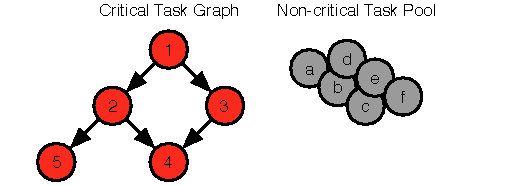
\includegraphics{figures/schedule-tg}} \\
\subfloat[]{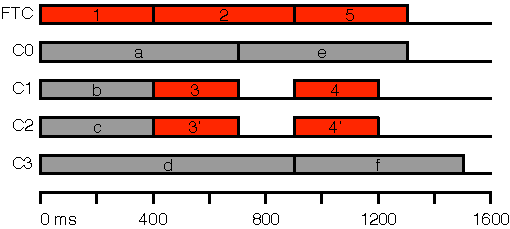
\includegraphics{figures/schedule-nodcc}} \\
\subfloat[]{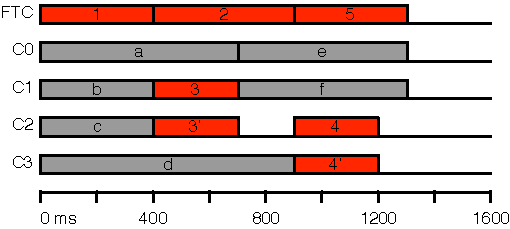
\includegraphics{figures/schedule-dcc}}
\caption[An example task graph for a mixed-criticality system]{(a) The task graph for a sequence of dependent critical tasks and a pool of non-critical tasks to be executed during the same window. (b) The tasks are mapped to a platform without DCC. (c) With DCC, NCT-f can begin 20 ms earlier.}
\label{f:schedule}
\end{figure}

\section{Fingerprinting Architecture}

\subsection{Overview}

The rest of this section will be organized as follows:
\begin{itemize}

\item{List the requirements a fault tolerant mechanism (FTM) should have in the context of an MPSoC with several independent cores.}
\item{Present the main components of the hardware platform.}
\item{Present the organization of a flexible software architecture.}
\item{Examine how each of the requirements is addressed with the high level specification in mind.}
\end{itemize}



\subsection{System Requirements}
This architecture aims to showcase the features of a fault tolerance mechanism that is purposefully suited to the scenario of a multicore RISC processor that uses some combination of specialized hardware and software to ensure predictable and dependable behaviour for mixed criticality applications. Examples of such systems have been discussed in the previous two sections. The future of software designs for such platforms is projected to involve the automatic generation of code as an optimization problem using platform models and various system requirements. This fault tolerant mechanism should therefore have a few basic properties:
\begin{itemize}
\item{Area overhead should be kept to a minimum and must be competitive with DMR or nMR}
\item{Any additional hardware should be scalable with the number of cores in a platform.}
\item{The system should not be dependent on network or bus topology}
\item{Monitoring of the execution stream or other core state information should be implemented in hardware and off the critical data path}
\item{The relative amount of data required to verify correct execution should be small compared to other system bus or network traffic. }
\item{Parameters related to reliability that impact the previously listed properties should be tunable. Tunability will minimize restrictions on the model-based design space exploration when generating optimized application code for a platform.}
\item{At least one agent in the system is permanently reliable and is responsible for monitoring less reliable agents}
\item{There should be a strategy for impeding the propagation of errors to other concurrent tasks on the core or elsewhere in the system}
\item{There should be a path to support the development of low cost checkpointing strategies}
\item{The system should bear some resemblance to DMR as a well established path to certification already exists}
\item{Minimal restrictions should be placed on the software organization in terms of scheduling}
\end{itemize}

\subsection{Hardware Architecture}

The baseline platform in Figure \ref{f:arch} consists of the following elements:
\begin{itemize}
\item{Two cores capable of executing non-critical tasks independently and of loosely synchronizing and executing the same critical tasks in parallel}
\item{Local scratchpads with identical addresses. The scratchpads are currently reserved for critical task stacks and input data however more complex dynamic allocations could be used. }
\item{DMA that can access the scratchpads and main memory. The monitor core is able to set the DMA units}
\item{Fingerprinting units that monitor each core}
\item{A specialized comparator core for collecting and comparing fingerprints from each core}
\item{A monitor core that is assumed to be made reliable through other permanent internal mechanisms that are not visible to the rest of the system (such as DMR). The monitor core is responsible for scheduling tasks and receives updates from the comparator core upon failure or success of a fingerprinted task.}
\end{itemize}


The general control flow for the system is depicted in Figure \ref{f:control_flow}.
	First, the Monitor task on the FTC \encircle{1}~assigns a pair of redundant critical tasks (SW) to two cores.
	This task is executed inside of a wrapper that \encircle{2}~sets up the fingerprinting unit (FP), requesting the software-specified fingerprinting block size for this task.
	Next, \encircle{3}~the task begins, prompting \encircle{4}~the fingerprinting unit to notify the comparator that fingerprint generation has started.
	While the task executes, \encircle{5}~fingerprints are generated and sent to the comparator.
	%As matching fingerprints arrive from the redundant critical task, the comparator compares them.
	As matching fingerprints arrive from the redundant critical task, they are checked by the comparator.
	In the meantime, speculative changes to state are quarantined in a scratch-pad memory (SPM) managed by the Monitor task on the FTC, with the assistance of DMA.
	
	If there is an interrupt and a higher-priority critical needs to execute, fingerprinting \encircle{6}~is paused, and a context switch performed.
	When the higher priority task finishes, control is returned to the original critical task, and fingerprinting is \encircle{7}~resumed.
	%The fingerprinting unit itself need not be aware that this has occurred (Section~\ref{s:hwsw:fingeprinting}).
	The comparator does not require notification that this has occurred.
	The critical task will eventually \encircle{8}~notify the fingerprinting unit that  the task has ended.
	The fingerprinting unit \encircle{9}~communicates this to the comparator, which then \encircle{10}~forwards final voting results to the monitor task. In the case of mismatched fingerprints, the comparator notifies the MC immediately.
%	If there has been an error, the monitor \encircle{11}~communicates this back to software (likely through the operating system) so that corrective action can be taken.
	If there has been an error, the monitor \encircle{11}~ should initiate a contingency schedule so that corrective action can be taken \cite{bolchini2013reliability}.
\begin{figure}[h]
\centering
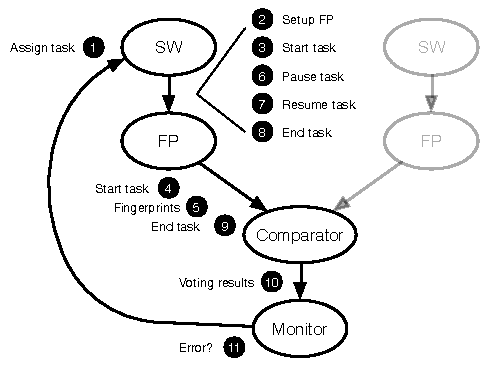
\includegraphics[scale=1.3]{Figures/interfaces}
\caption{System view of hardware platform.}
\label{f:control_flow}
\end{figure}

\subsection{Software Architecture}
 
This section explores the system-wide architectural implications that may arise in the software design due to the limitation of hardware resources and the fundamental requirement of fingerprinting that a task can be deterministically executed on separate cores not just in terms of the result produced but at the fine grain of individual store commands. These issues, pertaining to high level software design, will not be explored in any further detail in this work. However, they present interesting directions to explore in future work.

\subsubsection{Fingerprint task IDs}
Although a more comprehensive justification for the features of the software architecture must wait until the hardware constraints have been explored in more detail, the general organization of critical tasks across the system can still be provided. To begin with, there must be the definition of system wide fingerprint task IDs (FIDs). The maximum number of FIDs will be constrained by the fingerprinting hardware available in the system. This constraint leads naturally to the worry that more critical tasks exist than there are FIDs, making it impossible to statically assign a single FID to each critical function. The assignment of FIDs must be taken into account as another parameter when developing a schedule for the system. This can be easily achieved in a schedule with non-preemptive execution of critical tasks. A different strategy is required in systems where a fingerprinted task may be preempted.

A \emph{fingerprinting window} represents a certain mapping of FIDs to critical tasks. A fingerprinting window can be very short or very long and is meant to organize the assignment of FIDs to guarantee that all critical tasks concurrently executing in a system have an FID available to them. It can represent a static assignment or a static series of assignments. Suppose that the capacity of the system is \emph{n} FIDs. This means that at any given point in time, the comparator hardware is only able to maintain information on \emph{n} tasks at a time. In a system where critical tasks cannot be preempted (not an unreasonable assumption in highly critical real-time systems with very precise deadlines) this is very simple to do, especially if the number of regular cores $p \leq 2n$. For instance, suppose $n = 16$. In a non-preemptive schedule, it is possible to have 16 \emph{pairs} of cores executing a critical task simultaneously.

The fingerprinting window becomes more restrictive in a system that allows preemption of fingerprinted tasks. In this case, more than one critical task may be simultaneously executing on each core. Therefore care must be taken that an FID is available for any task requiring fingerprinting. We can compromise by placing some restrictions on the servicing of these tasks into set frames where no more than 16 functions have access to the fingerprinting resources at a time. Resource sharing in multicore systems with real-time deadlines is an ongoing area of research. Frames or windows are a common theme in establishing predictability of execution making this an approach that could easily be integrated into such a system.

The assignment of functions to FIDs as well as the assignment of FID/function pairs to cores is handled by the reliable monitor core. The monitor core has unique access to the input data for the critical task. Memory protection must be used to guarantee that only the monitor can initiate writes to these addresses (either directly or using DMA). The monitor can then use DMA to prepare the state on the scratchpad on each local core, including input data, function code location, and FID. 

\subsubsection{Deterministic execution}

The \emph{scratchpad resources} of each core are important to ensuring deterministic execution of redundant tasks as well as another limited resource that must be taken into account when scheduling. Both these issues will now be elaborated on. The availability of a stripped down memory virtualization capability may also be required as a practical matter depending on the specific architecture and compiler. 

The \emph{deterministic execution} of a function in a system without virtual memory support and high level process services from the OS is not an unsolvable or even particularly complicated problem but it is also not a forgiving one. Depending on the processor architecture and compiler options available, it can be tricky to generate machine code for one core that can be executed without-modification by another core.

The goal is to allow the compilation of deterministically executing of code without the availability of position independent code options (-fpic) that can be run by any core in the system without modifying the compiler. The issue is that if the code references global variables, then only one copy of the variable exists. There are two less than ideal solutions to this problem. The first is to rewrite the code so that all recurring global state variables used by a function are accessed through pointers passed into the context as function arguments and therefore placed on the stack, and then popped off the stack back into main memory at the end of the execution. The addresses of these variables will never be compiled directly into the machine code of the critical tasks. This can obviously be cumbersome, especially considering that code generated from models may not behave this way. The second is to place copies of global variables in the local scratchpads and use \emph{memory virtualization} to ensure that the references to these variables are rerouted to the local copy.

In order to have strictly deterministic execution of regularly compiled code, all store addresses and data (at a minimum) must match for the entirety of the fingerprinted interval. As a result, it is necessary that the stack pointers match from the beginning of fingerprinting. It is also required that same copy of the code is run from the same address on both cores so that all return addresses pushed onto the stack are matching. It bears repeating that these conditions are restrictive in terms of the way code must be written to guarantee deterministic execution \emph{without} the availability of memory virtualization in a bare-metal (RTOS-based) system. It also bears repeating that virtualization hardware is very central to the design of hypervisors and should be fairly common in embedded real-time MPSoCs. We have include a low cost uTLB for minimal virtualization of scratchpad addressing.

\subsubsection{Fault containment strategies}
	While executing a safety-critical task, the output from unreliable cores are prevented from making changes to external state until such changes have been verified through fingerprint comparison. 
	There are two potential approaches. Firstly, the use of local scratchpad memories or locked caches can be used to store temporary copies of data. 
	Alternatively, several redundant copies could be kept in main memory \cite{dobel2012operating}. 
	In either case, there is a probability that the setting of the MPU is itself corrupted. Either a fault tolerant core should manage memory protection to guarantee that erroneous write addresses cannot corrupt data outside of the current task. In \cite{huang2014framework} it is suggested that a probabilistic argument can be made about the likelihood of that specific task failing to determine whether or not this function must be moved to an FTC. 
	There is no way to guarantee that a failure does not corrupt other tasks concurrently stored on the local memory resource if a non reliable core manages its own local memory protection since the memory protection itself could be erroneously set. 
	In the case of several copies in main memory a single core could reasonably be expected to control a global MPU. 
	We have yet to integrate memory protection strategies into our software development but note that work exists to address certifiable memory partitioning in mixed criticality multicore systems using hypervisors \cite{perez2013safety}.
	
	Advantages of using a scratchpad include not requiring several copies of the data and stack for a critical task in main memory as well as other known benefits including including more deterministic execution \cite{suhendra2005wcet} and energy efficiency \cite{steinke2002assigning}. 
	The difficulty is that there is now another limited resource to be allocated and that will affect scheduling. Furthermore, programs that operate on large data arrays provide problems for scratchpad allocation \cite{francesco2004integrated}. 
	By contrast, keeping several copies in main memory solves many of these problems, however, introduces problems of scalable determinism as the number of cores increases and interference affects memory response times \cite{abel2013impact}. 
	For these reasons, and due to promising work that suggests many of these large data processing algorithms will be shifted to fault tolerant tightly coupled processor arrays \cite{nelis2014challenge,lari2014massively,ferreira2014adaptive}, we will use scratchpads.
	\begin{figure}[h]
\centering
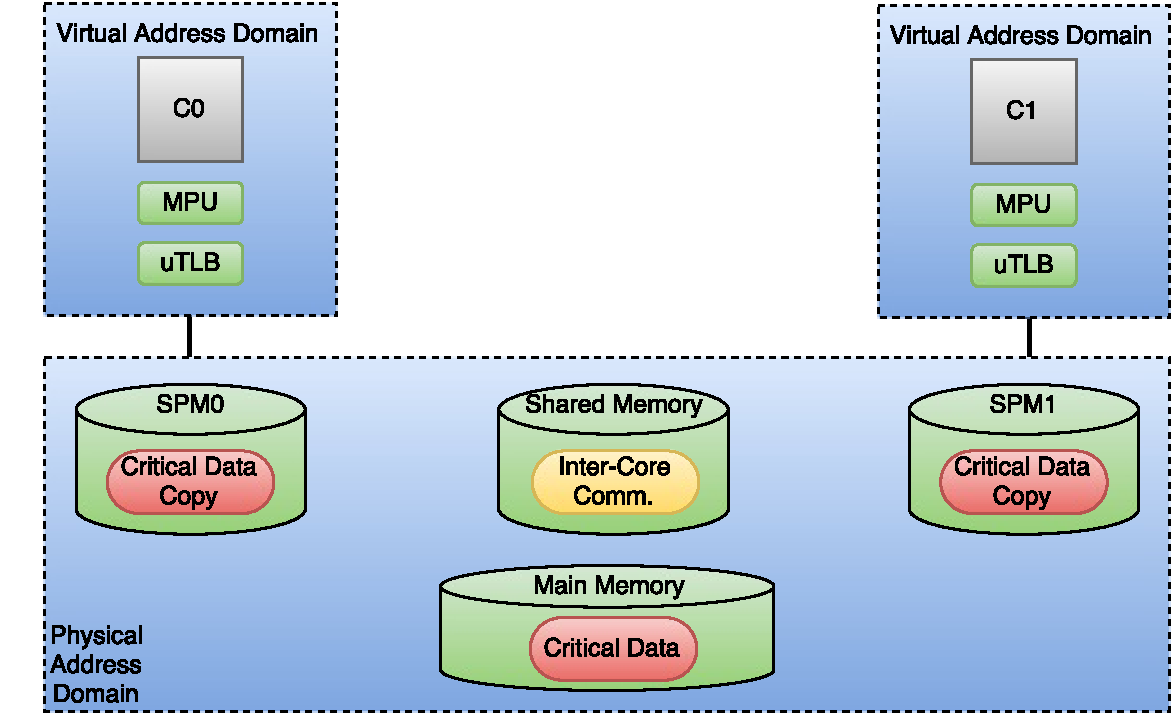
\includegraphics[scale=1]{Figures/sor}
\caption[Memory protection and fault containment]{Memory protection could be used to quarantine changes to critical state in the scratchpad. Less space is required in main memory since the replicas only exist temporarily in the scratchpad. The fingerprint units (FP) base their calculations on the virtual addresses.}
\label{f:sor}
\end{figure}
	Figure \ref{f:sor} shows how memory partitioning can be used to create temporary copies of critical data in scratchpads and protect the original in main memory. It should not be possible for the plain cores to access protected data directly.
	Both the critical task stacks and any input data must be protected.
	
	The software is organized using generic critical task wrappers that can execute an arbitrary function with an arbitrary FID.
	The wrapper tasks will either determine from a static schedule or from a message from an FTC when they should execute, what the identify of the critical function is, and where to find its arguments. 
	There should be enough wrapper functions to support the maximum number of concurrent critical tasks expected to run. 
	If there is sufficient room in the scratchpad to store all of the stacks then they can be statically allocated. 
	Otherwise, the stacks for the tasks can be copied into the scratchpad and the uTLB used for address translation. 
	In order for fingerprinting to operate correctly, the virtual addresses of the stack must be identical on both cores. 
%	We simplify the situation by making the scratchpads only addressable locally, and giving them all identical addresses. 
	%This eliminates the need for address translation with static allocation of the scratchpad . 
	The FTC is able to differentiate between these scratchpads using a local single threaded DMA controller.




\subsubsection{Preempting Critical Tasks}
\label{s:hwsw:preemption}

	At times it may be necessary for one critical task to preempt another.
	In the context of fingerprinting, this presents additional challenges:
		the fingerprinting of the preempted task must not be disrupted, but the fingerprinting logic must be available for the new task.
	The simplest solution to the problem is to have the software notify the hardware when it begins servicing an interrupt. 
	The problem arises that there is no way for communication between software and hardware to occur without the software corrupting its own context (it must load the address of the hardware into a register). 
	We propose a convention whereby the fingerprinting hardware is able to roll back its calculations by one iteration, thus allowing a single store instruction to be executed without corrupting the fingerprint. 
	When an interrupt occurs, the initial context saving assembly routine is modified to store exactly one register onto the stack, and then this register is used to load the address of the fingerprint unit pause strobe. 
	The fingerprint unit rolls back its calculation by one iteration when it receives the pause strobe. 
	When the fingerprint process resumes, the execution streams from both cores will still match.
	
	It is possible to imagine more complex message passing between the OS and the fingerprinting unit once fingerprinting has been successfully paused. 
	For instance, the fingerprinting unit currently only supports rate monotonic scheduling and stores paused task context on a stack. 
	It is reasonable for the OS to pass messages to the fingerprinting to notify it which task is being resumed and for the hardware stack to be replaced by a more flexible data structure. 
	There are potential issues here in that the unreliable core is now passing information to the FP unit that may affect the fingerprinting of several tasks if it is not done properly. 
	We do not explore this issue in any greater detail but note that this behaviour is easily supported by the hardware should it be desired.
In order for the system to provide fail operational capabilities it must be shown that any erroneous executions are not able to contaminate other tasks or applications. It will be necessary to implement a fine grained memory protection strategy. This aspect of the problem has not yet been explored for this project. 

 \chapter{Structure of Software Services} % Main chapter title

\label{Chapter2} % For referencing the chapter elsewhere, use \ref{Chapter1} 

\lhead{Chapter 2. \emph{Structure of Software Services}} % This is for the header on each page - perhaps a shortened title

%----------------------------------------------------------------------------------------

\section{Introduction}

This chapter will present in some detail the structure of the code on each core and how basic services such as inter-core communications, synchronization, task assignments, and fingerprinting are implemented. The data structures for organizing fingerprinting task IDs (FIDs) across the system and how they are communicated to hardware will be shown. The reader is referred back to Figure \ref{f:control_flow} as a reference. Even the simple template code can be difficult to interpret because it is distributed across three cores. Figure \ref{f:control_flow} provides a chronological view of the procedure for dynamic scheduling of a critical task on plain cores by the monitor. The important pieces of code associated with each of these steps will now be discussed.

\begin{figure}
\centering
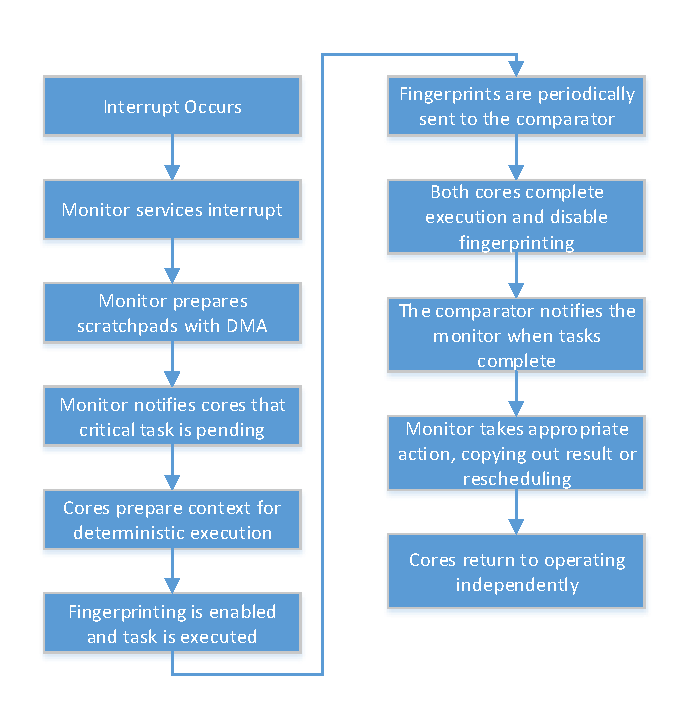
\includegraphics[scale=0.8]{Figures/control_flow}
\caption[Example of directory partitioning]{Example of directory partitioning: Task 0 reserves enough space to maintain a circular queue of size 50. Task 1 reserves a queue of size 25. And Task 2 uses the remainder of available memory.}
\label{f:control_flow}
\end{figure}


\section{Inter-core communication}

As we are dealing with a very simple real-time operating system (RTOS), it is not an easy task to implement a software only solution for message passing between cores. It is not possible to share key data structures such as event-control blocks (ECBs) between cores. An ECB is the basic data structure used by the uC/OS-II RTOS (uCOS from here on) to define mutexes, semaphores, event flags, and queues. Since the RTOS is not built to be able to share ECBs between different instances on different cores it is necessary to develop another solution. Fortunately it is fairly straightforward to create custom memory mappings with soft cores on the FPGA to provide hardware implemented message passing structures.


A 1kB region of memory is reserved for the passing of messages between cores. Furthermore, each core has a register that is addressable by the other cores that triggers an interrupt. The size of the shared memory region can be adjusted if necessary. It is also assumed that each piece of information in the shared memory at any given time is only written by one core. Access to shared memory is controlled with a hardware mutex. Listing \ref{l:mon_init} shows how the monitor core initializes certain system variables and notifies the other cores. The initialization of the plain cores is stalled until the monitor is able to set up certain global variables.

 \begin{lstlisting}[frame=single,language=C,label=l:mon_init,caption={[Monitor passes messages to other cores]The monitor core aquires a hardware mutex and uses shared memory to pass messages to the other cores}] 
 CriticalFunctionPointers* cp = (CriticalFunctionPointers*) SHARED_MEMORY_BASE;
 //Acquire the mutex
altera_avalon_mutex_lock(mutex, 1);
{
	//Set some initial start up values
	cp->critical = critical_task;
	cp->preempt = qsort_test;
	//Notify other cores that initialization is complete
	cp->init_complete = 1;
}//release the mutex
altera_avalon_mutex_unlock(mutex);
 \end{lstlisting}
Meanwhile the plain cores wait for the cp$\rightarrow$ init\_complete variable to change before proceeding with their initialization in Listing \ref{l:core_init}.

\begin{lstlisting}[frame=single,language=C,label=l:core_init,caption={[Plain core startup synchronization]Plain core waits for the initialization by the monitor to finish before updating the variables}] 
//The plain cores wait on the init_complete variable
while(cp->init_complete == 0);
altera_avalon_mutex_lock(mutex, 1);			
{
	//They load the values placed in shared memory by the monitor
	ct = cp->critical;
	pt = cp->preempt;
}
altera_avalon_mutex_unlock(mutex);		
\end{lstlisting}


In this example, the plain cores are at the beginning of their code and are using a spin lock because they all must wait until the monitor has reached a certain point in its startup before they can continue and \emph{no other work} can be done since this is the startup routine. However, \emph{all subsequent} communication between the monitor and the cores will be \emph{interrupt driven}. As previously mentioned, each core is capable of interrupting the execution of the others. Currently, communication is only one way: from the monitor to the plain cores. Listing \ref{l:mon_irq_send} shows the monitor code for causing an interrupt in the other cores and Listing \ref{l:cpu_irq} shows the response from the plain core. This method can be generalized by including a message type header at the beginning of shared memory in order to pass several different types of information. In this example it is assumed that only one type of message passes from monitor to other cores.

\begin{lstlisting}[frame=single,language=C,label=l:mon_irq_send,caption={[Monitor message passing to plain cores]The monitor core puts a message in the shared memory region and then writes to the ISR pointer variables\, triggering interrupts in the other cores.}]
int *isr_0_ptr = (int *) PROCESSOR0_0_CPU_IRQ_0_BASE;
int *isr_1_ptr = (int *) PROCESSOR1_0_CPU_IRQ_0_BASE;	
altera_avalon_mutex_lock(mutex, 1);
{
	cp->task_id0 = (5);
	cp->task_id1 = (5);
	*isr_1_ptr = 1;
	*isr_0_ptr = 1;
}
altera_avalon_mutex_unlock(mutex);
\end{lstlisting}

\begin{lstlisting}[frame=single,language=C,label=l:cpu_irq,caption={[Plain cores retrieve arguments from shared memory]The plain cores handle the interrupt and retrieve the necessary information.}]
static void handle_cpu0_interrupt(void* context) {
	unsigned short task_id;
	altera_avalon_mutex_lock(mutex, 1);
	{
		CriticalFunctionPointers* cp = 
		    (CriticalFunctionPointers*)SHARED_MEMORY_BASE;
		task_id = cp->task_id0;
		*isr_0_ptr = 0;
	}
	altera_avalon_mutex_unlock(mutex);
	if(task_id == CRITICAL_TASK_PRIORITY)
		OSSemPost(mbox);
}
\end{lstlisting}

\section{Initializing and communicating with the Comparator core}

As was already discussed in Chapter \ref{Chapter1}, the monitor core is responsible for organizing the mapping of FIDs to actual critical functions. It is not necessary for this mapping to be static and it is not possible if there are more functions than FIDs. There are two pieces of information required by the comparator in order for it to correctly interpret messages from the fingerprinting units: which core is executing a given FID, and how to partition the local memory space between tasks for the storage of fingerprints.

\subsection{The core assignment table}

The \emph{core assignment table} (CAT) is a mapping of a \emph{physical core ID} (PCID) to a \emph{virtual core ID} (VCID). The PCID is a 4 bit number that is assigned uniquely to each core and fingerprinting unit. The comparator in the current implementation is limited to the comparison of two cores and is not capable of error correction through voting. Furthermore, the FID is a 4 bit number allowing up to 16 concurrent tasks to be fingerprinted. Since each FID can only be executing on two cores at a time, a table keeps track of which two cores are executing each task. An example is shown in Table \ref{t:cat}. Here, the task with FID 0 is defined to execute on cores 0 and 1. The task with FID 1 is defined to execute on cores 1 and 3. The \emph{actual function} associated with each FID can change without changing the CAT. The equivalent code for programming the hardware is shown in Listing \ref{l:cat}.


\begin{table}
\centering
    \begin{tabular}{| l | l | l  |}
    \hline
    Task & PCID 0 & PCID 1\\ \hline
    0 & 0 & 1\\ \hline
    1 & 1 & 3\\ \hline
    2 & 2 & 0\\ \hline
    3 & 2 & 3\\ \hline
    \end{tabular}
    \caption[An example core assignment table.]{An example core assignment table. Each row is associated with a task shown in this picture for demonstration purposes; the real table only has two columns and the task is implicitly defined by the index number. }
    \label{t:cat}
\end{table}


\begin{lstlisting}[frame=single,language=C,label=l:cat,caption=The monitor programs the CAT in the comparator.]
Core_Assignment_Table ca;
//ca.table[VCID][FID] = PCID
ca.table[0][0] = 0;
ca.table[1][0] = 1;
ca.table[0][1] = 1;
ca.table[1][1] = 3;
ca.table[0][2] = 2;
ca.table[1][2] = 0;
ca.table[0][3] = 2;
ca.table[1][3] = 3;
set_core_assignment_table(&ca);
}
\end{lstlisting}

\subsection{Initializing the directory}

The next step for the monitor is to define the partitioning of the comparator's local memory space to store fingerprints. In the current implementation, the comparator has capacity to store 512 fingerprints. The 512 spaces can be divided amongst the 16 FIDs in arbitrarily sized circular queues. For instance, suppose FID 1 is associated with a function known to produce a single fingerprint. It is possible to reserve a single memory location for this task. Suppose FID 1 is known to produce over a thousand fingerprints. It may be prudent to subdivide this task into several fingerprinting intervals. However it is also possible to reserve a queue of size 50 for this task if it can be shown that the fingerprint buffer will not overflow (due to one core executing significantly faster than the other). Development of a feedback mechanism to slow down a core that is pulling too far ahead of its partner core without explicit software barriers is under way. One method of setting the directory according to this example is shown in Listing \ref{l:dir_init}. It is crucial to \emph{never} make changes to the directory structure while any tasks are being fingerprinted. For now it is the case that both virtual cores require the same directory layout, however it is still necessary to set the directory for each core individually. An example of directory partitioning is shown in Figure \ref{f:directory}

\begin{lstlisting}[frame=single,language=C,label=l:dir_init,caption=Initializing the Comparator directory.]
Directory_Init_Struct d;
//Set the directory for each virtual core
for(i = 0; i < 2; i++){
	d.core_id = i;
	//Task 0 requires a single slot
	d.key = 0;
	d.start_ptr = 0;
	d.end_ptr = 0;
	set_task_directory(&d);
	//task 1 requires several slots
	d.start_ptr = 1;
	d.end_ptr = 51;
	set_task_directory(&d);
}
\end{lstlisting}


\begin{figure}[ht]
\centering
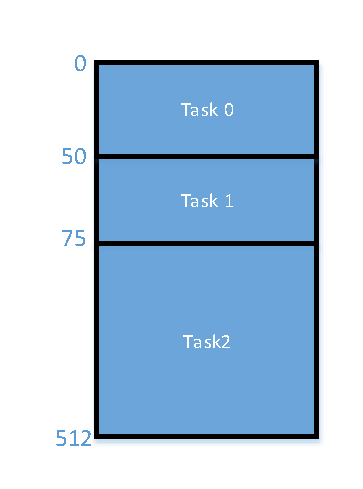
\includegraphics[scale=0.8]{Figures/directory}
\caption[Example of directory partitioning]{Example of directory partitioning: Task 0 reserves enough space to maintain a circular queue of size 50. Task 1 reserves a queue of size 25. And Task 2 uses the remainder of available memory.}
\label{f:directory}
\end{figure}

\section{Initiating a critical task with the Monitor}
Once the comparator has been properly initialized, the Monitor can begin to request the execution of critical tasks from the plain cores. Presumably the request from the monitor would itself be triggered by some interrupt. The monitor will then acquire the hardware mutex, transfer any necessary information into the scratchpads of the cores using DMA, place a pointer to the function, the FID, and any other arguments that can be user defined in shared memory, and interrupt the cores. Listing \ref{l:mon_task} shows how the monitor might initiate a critical task.
\begin{lstlisting}[frame=single,language=C,label=l:mon_task,caption={[Mointor initiates a critical task on plain cores]The monitor requests cores 0 and 1 to begin executing a function called critical\_task with FID 0.}]
altera_avalon_mutex_lock(mutex, 1);
{
	cp->function[0] = critical_task;
	cp->function[1] = critical_task;	
	cp->fid[0] = (0);
	cp->fid[1] = (0);	
	cp->blocksize[0] = 0x5ff;
	cp->blocksize[1] = 0x5ff;
	cp->args[0] = (void*)function_args;
	cp->args[1] = (void*)function_args;
	*irq_1_ptr = 1;
	*irq_0_ptr = 1;
}
altera_avalon_mutex_unlock(mutex);
\end{lstlisting}
\section{Executing a critical task with fingerprinting}
uCOS has a capacity for 256 tasks with priorities 0-255. It is not possible for two tasks to have the same priority. The simplest thing to do is to reserve tasks 0-15 for fingerprinting. Each OS task (OST) is assigned a generic wrapper that will execute an arbitrary function associated with the given FID. The identities of the function and FID are passed by the comparator as shown in Listing \ref{l:mon_task}. More flexible and powerful message passing schemes can be implemented. The method of responding to a request from the monitor is shown in listing \ref{l:cpu_response}. Some parts of the code not essential to the current discussion have been omitted.
\begin{lstlisting}[frame=single,language=C,label=l:cpu_response,caption=Plain core 0 responds to the request from the monitor.]
void (*critical_task)(void*);
int blocksize;
//Interrupt handler
static void handle_cpu0_interrupt(void* context) {
	unsigned short task_id;
	altera_avalon_mutex_lock(mutex, 1);
	{
        CriticalFunctionPointers* cp = 
            (CriticalFunctionPointers*)SHARED_MEMORY_BASE;
        //retrieve the FID of the task
		task_id = cp->fid[0];
		//retrieve the address of the function
		critical_task = cp->function[0]
		//retrieve the fingerprinting block size
		blocksize = cp->blocksize[0];
		//reset the IRQ
		*irq_0_ptr = 0;
	}
	altera_avalon_mutex_unlock(mutex);
	//Activate the appropriate OS task
	if(task_id == PRIORITY_0)
		OSSemPost(sem_0);
	else if(task_id == PRIORITY_1)
		OSSemPost(sem_1);
}

//The tlb must be used for global variable references
void init_tlb(){
	set_cputable_entry(1, GLOBAL_VARIABLE_SECTION);
	set_spmtable_entry(1, TLB_BASE);

	//Enable the translations
	set_enable(0x2);

}

//The critical task wrapper:
INT8U err;
void critical_task_wrapper(void* pdata){
	int* p = pdata;
    //The priority is assigned to the task when created by the OS
	int priority = *p;
	while(1){
		//A single task wrapper can be written for all priorities using
		//conditional waiting
		if(priority == PRIORITY_0)
			OSSemPend(sem_0, 0, &err);
		else if(priority == PRIORITY_1)
			OSSemPend(sem_1, 0, &err);
	    
	    //the critical task address is loaded onto the stack
	    void (*pt)(int) = critical_task;
		//the block size is forwarded to the fingerprint unit	    
	    fprint_set_block_size(blocksize);
	    //The TLB is initialized with the proper translation table
		init_tlb();
		//The TLB is enabled
	    enable_tlb();
		long registers[8];
		//The callee saved registers must be pushed to the stack
		// and set to 0
		context_switch(registers);
		//The global pointer is set to match the monitor core
		set_gp();
		//The critical task is executed
		critical_task(&args);
		//Restore the local global pointer register
		restore_gp();
		//Restore the callee saved registers
		context_restore(registers);
		//Turn off translation
		disable_tlb();
	}
}
\end{lstlisting}

There are several important things that happen in this code. First is the interrupt handler. This retrieves the FID and the function pointer from the shared memory region. It also retrieves the blocksize that sets the number of stores used by the fingerprint unit to calculate each fingerprint (where the size of the block affects the hamming distance and guaranteed error coverage provided by the CRC algorithm). It then signals the appropriate task wrapper based on the value of the FID. The task wrapper is the same generic wrapper for all critical tasks. Each wrapper is statically assigned a priority by the OS during startup. Each wrapper waits on its own signal. When the signal arrives from the interrupt handler, the wrapper then does several things before calling the task: it turns on the TLB, it saves and resets the context, it changes the global pointer, and then it finally calls the critical task. Recall that memory translation, GP substitution, and the setting of callee saved registers to zero prior to initiating fingerprinting are required to ensure \emph{deterministic execution}. Also note that changes are made to the initial interrupt context save routine in order to restore the GP for interrupt handlers so that these will not be broken if interrupts are not disabled during the critical task.

There is one more layer to get to the proper critical function. The issue is that fingerprinting must be enabled and disabled without storing the return address of the local wrapper function. This return address would not match on the different cores. Therefore a \emph{wrapper within the wrapper} is required. The code that enables and disables fingerprinting must be part of the shared code. Suppose that the critical task in question was an FSM control for the shift logic in a car. When the critical task is called from the wrapper in Listing \ref{l:cpu_response}, it takes the form of Listing \ref{l:critical_task}. This code, including the FSM function, are compiled for the Monitor to ensure the location of global variables are in the section of memory being translated by the TLB.

\begin{lstlisting}[frame=single,language=C,label=l:critical_task,caption=The inner layer wrapper.]
void critical_task(void* args){
	int priority = *(int *)args;
	enable_fprint_task(priority);
	    ShiftLogic_step();
	disable_fprint_task(priority);
}
\end{lstlisting}

All other activity between the fingerprinting units themselves and the comparator are invisible to the software. When the result of a comparison is ready, the Monitor is notified via interrupt. As shown in Listing \ref{l:mon_comp_int}, the Monitor uses simple functions to retrieve a status update from the Comparator. Depending on the program, further actions can be taken. It remains to be done to develop a generalized framework across the system for killing and restarting failed tasks.

\begin{lstlisting}[frame=single,language=C,label=l:mon_comp_int,caption=The monitor interrupt handler for the comparator]
static void handle_comp_interrupt(void* context) {
	int endstate[10];
	Fprint_Status status;
	fprint_status(&status);
	...
}
\end{lstlisting} 
 
\chapter{Hardware Design} % Main chapter title

\label{Chapter3} % For referencing the chapter elsewhere, use \ref{Chapter1} 

\lhead{Chapter 3. \emph{Hardware Design}} % This is for the header on each page - perhaps a shortened title

There are two hardware components required for fingerprinting: the fingerprinting unit itself and the centralized comparator. The fingerprint unit must passively monitor the data bus of a core to compute fingerprints and periodically send these fingerprints to the comparator. The comparator must pool and organize fingerprints collected from all the cores and compare them to decide if the system is operating correctly. The comparator must then notify the monitor core upon the successful completion of a task or if an error has been detected. Three interfaces must be specified: the cores to the fingerprint unit, the fingerprint unit to the comparator, and the comparator to the monitor. This section will describe these interfaces as well as cover the mechanism by which rate monotonic (RM) scheduling is supported (i.e. preemption of fingerprinted tasks) and the internal microarchitectures of the fingerprint unit and the comparator.

\section{Fingerprinting Interfaces}
\subsection{Processor/Fingerprint Unit Interface}
Table \ref{t:fprint_reg} contains the list of registers in the fingerprint unit that can be written by the processor it is attached to. Note that all address offsets are given from the perspective of the sender. The sender address offset is always shifted left by two bits compared to the offset the receiver uses. The current state register bitfield is defined in Table \ref{t:cs_bitfield}.
\begin{table}
\centering
    \begin{tabular}{| l | l | l  | p{6cm} |}
    \hline
    Register & RW & Offset & Function\\ \hline
    Current State (CS) & W & 0x0 & Used to enable and disable fingerprinting\\ \hline
    Block size (BS) & RW & 0x10 & The BS register contains the size of a fingerprinting block for the current task\\ \hline
    Pause  & R & 0x8 & The pause register is used by the interrupt trap to signal that the current task should pause its fingerprinting. The value read has no meaning.\\ \hline
    Unpause & R & 0xc & The unpause register is used by the interrupt trap to signal that the most recently paused task should resume fingerprinting. The value read has no meaning.\\ \hline
    \end{tabular}
    \caption{Fingerprint unit control registers}
    \label{t:fprint_reg}
\end{table}


\begin{table}
\centering
    \begin{tabular}{| l | l | l | p{6cm} |}
    \hline
    Name & Offset & Size(bits) & Function\\ \hline
    FID & 0x0 & 4 & The FID of the task beginning or ending fingerprinting.\\ \hline
    Enable bit & 0x4 & 1 & The enable bit signals whether fingerprinting is beginning or ending.\\ \hline
    \end{tabular}
    \caption{Current state register bitfield.}
    \label{t:cs_bitfield}
\end{table}

The functions used for this purpose are:
\begin{itemize}
\item{enable\_fprint\_task(int FID): begin fingerprinting on the given core a task with FID.} 
\item{disable\_fprint\_task(int FID): end fingerprinting on the given core a task with FID.}
\item{fprint\_set\_block\_size(int size): set the block size for the task beginning fingerprinting. Set prior to enabling fingerprinting.}
\end{itemize}

\emph{Block size:} A default value of 0xFFF is currently provided for the fingerprint unit. The block size \emph{MUST} be odd to function correctly. In anticipation of future work exploring the fingerprinting of both store and load instructions, the counter is currently set to increment by 2 since load instructions contribute half as many bits as store instructions (only the address is used). A value of 0xFFF = 4095 signifies that 2048 stores will be used to calculate a fingerprint. Each store contains 59 bits (27 address and 32 data bits). This means that each 32 bit fingerprint compresses 120832 bits of execution stream resulting in 3776x compression. A table of polynomials including block sizes over which a given hamming distance is achieved is provided in \cite{koopman200232}.
\begin{figure}
\centering
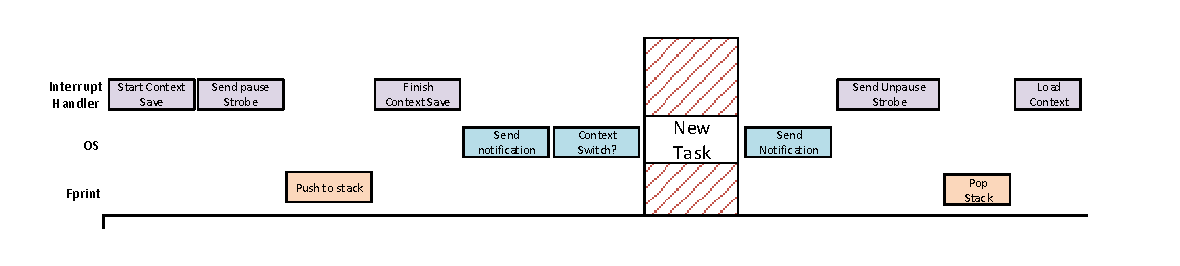
\includegraphics[scale=0.8]{Figures/interrupt}
\caption[Preemption of a fingerprinted task]{Preempting a fingerprinted task without corrupting the fingerprint. The low level assembly interrupt handler and the OS interrupt wrappers are depicted separately.}
\label{f:int}
\end{figure}
\emph{Pausing: } 	At times it may be necessary for one critical task to preempt another. 
	In the context of fingerprinting, this presents additional challenges:
		the fingerprinting of the preempted task must not be disrupted, but the fingerprinting logic must be available for the new task.
	Figure \ref{f:int} shows the procedure.
	First, the interrupt vector responsible for context saving located in the BSP is modified to send a strobe to the fingerprint unit notifying it that it should stop fingerprinting.



	The problem arises that there is no way for communication between software and hardware to occur without the software corrupting its own context (it must load the address of the hardware into a register). 
	We propose a convention whereby the fingerprinting hardware is able to roll back its calculations by one iteration, thus allowing a single store instruction to be executed without corrupting the fingerprint. 
	When an interrupt occurs, the initial context saving assembly routine is modified to store exactly one register onto the stack, and then this register is used to load the address of the fingerprint unit pause strobe (Listing \ref{l:int_trap_st}). 
	
		\begin{lstlisting}[frame=single,language=C,label=l:int_trap_st,caption=The updated trap at the start of an interrupt.]
stw   ra,  0(sp)
movhi ra,  \%hi(0x8100000)
ori   ra,  ra, 8
ldw   ra,    0(ra)
stw   r1,   8(sp)
stw   r2,  12(sp)
...
\end{lstlisting}

	The fingerprint unit rolls back its calculation by one iteration when it receives the pause strobe. 
	Following this, the RTOS has its own interrupt wrapper functions. The OS notifies the fingerprint unit that it is about to call the context switch routine.
	If a higher priority task is ready, then it will execute in its entirety.
	When the context switch function finally returns, the OS again sends another notification to the fingerprint unit. 
	Finally an unpause strobe is included in the context restore vector in the BSP (Listing \ref{l:int_trap_ld}).
	\begin{lstlisting}[frame=single,language=C,label=l:int_trap_ld,caption=The updated trap at the end of an interrupt.]
movhi ra,  %hi(0x8100000)
ori   ra,  ra, 12
ldw   ra,    0(ra)
ldw   r5,  68(sp)
ldw   ea,  72(sp)  
ldw   ra,   0(sp)
...
\end{lstlisting} 
	The main purpose of the OS notification is to guard against unwanted behaviours that may arise due to nested interrupts. It is possible to imagine other types of communication passing between the OS and the fingerprinting unit once fingerprinting has been successfully paused. 
	For instance, the fingerprinting unit currently only supports rate monotonic scheduling and stores paused task context on a stack. 
	It is reasonable for the OS to pass messages to the fingerprinting to notify it which task is being resumed and for the hardware stack to be replaced by a more flexible data structure. 
	There are potential issues here in that the unreliable core is now passing information to the FP unit that may affect the fingerprinting of several tasks if it is not done properly. 
	We do not explore this issue in any greater detail but note that this behaviour is easily supported by the hardware should it be desired.
%
%
%
%Corrupting the context is not an issue at the end of the interrupt. The unpause strobe can simply be activated before loading back the original context. It must be the case that no interrupt related stores occur after the unpause strobe. If stack exceptions are enabled, for instance, the location of the pause strobe would have to be slightly altered. Listing \ref{l:int_trap_ld} shows the unpause strobe in the trap.
%
%
%The last thing that should be mentioned with respect to pausing is that there is also a uCOS wrapper that is executed prior to the user defined interrupt handler. This can be modified in future versions to send more information from the OS to the fingerprinting unit about the task to be resumed. Figure \ref{f:exception_flow} shows the software flow of exception handling in the Nios system. Once fingerprinting is paused, the OS Interrupt Exit function can be modified to send more details to the fingerprinting unit using as of yet unspecified control registers.

%\begin{figure}[h]
%\centering
%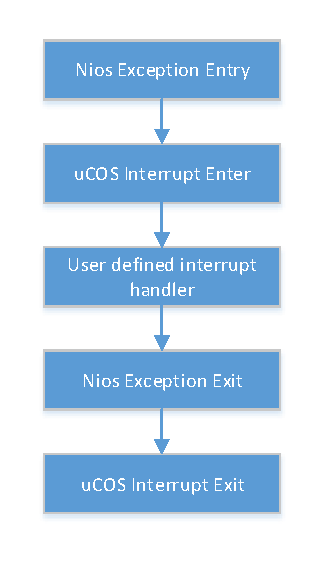
\includegraphics[scale=0.8]{Figures/exception_flow}
%\caption{Exception software flow in Nios II system.}
%\label{f:exception_flow}
%\end{figure}

\subsection{Fingerprint unit/Comparator Interface}
Messages are passed from the fingerprinting unit to the comparator when a task begins, when a fingerprint is complete, and when a task ends. The pausing of tasks is invisible to the comparator. Task begin/end messages can be sent in a single packet. Fingerprints require two packets to be sent to the comparator. The type of message being sent and the identity of the sender are encoded in the lower bits of the address. Table \ref{t:msg_format} shows the format for these messages. The size of each field could potentially be changed to satisfy different platform criteria. The messages could also be divided into two packets if the size of the offset becomes unreasonably large.
\begin{table}[h]
\centering
    \begin{tabular}{| l | l | l | l | l | }
    \hline
     & Base Address & Core ID & Message Type & Pad\\ \hline
    Message & 17 bits & 4 bits & 4 bits & 2 bits (0)\\ \hline
    \end{tabular}
    \caption{Message type format for sending messages from the fingerprint unit to the comparator.}
    \label{t:msg_format}
\end{table}
\begin{table}[ht]
\centering
    \begin{tabular}{| l | l |}
    \hline
    Message Type & Value\\ \hline
    Status update & 0\\ \hline
    Fingerprint & 4\\ \hline
    \end{tabular}
    \caption{Message type values for sending messages from the fingerprint unit to the comparator.}
    \label{t:msg_types}
\end{table}

The possible values for the current message types are shown in Table \ref{t:msg_types}. In the case of sending a fingerprint, it is necessary to break the 32 bit CRC up into two messages in order to be able to send the FID of the task that generated the fingerprint as well.  The format for sending fingerprints over two packets is shown in Table \ref{t:fprint_format}.

\begin{table}[h]
\centering
   \begin{tabular}{| l | l | l | l | }
    \hline
     & Partial Fingerprint & Packet & FID\\ \hline
    Lower half & 16 bits & 12b'0 & 4 bits\\ \hline
    Upper half & 16 bits & 12b'10 & 4 bits\\ \hline
    \end{tabular}
    \caption{Format for sending 32 bitfingerprints in 2 packets.}
    \label{t:fprint_format}
\end{table}


\subsection{Comparator/Monitor Interface}

Table \ref{t:comp_reg} contains the list of registers in the Comparator unit that can be accessed by the monitor core. The directory stores the offsets for start and end pointers of a circular queue and the addressing convention is given in Table \ref{t:dir_format}. The format for setting the core assignment table is shown in Table \ref{t:cat_format}. Each entry in the table is given by a unique address and addressing assumes that the size of the individual entry is 4 bytes even if the physical size of the memory is different (i.e. line 0 is at 0x0 and line 1 is at 0x4 regardless of the size of a line). Note that all address offsets are given from the perspective of the sender. The sender address offset is always shifted left by two bits compared to the offset the receiver uses.

The functions available to the monitor are:
\begin{itemize}
\item{fprint\_reset\_irq(void): Resets the status, fail and success register.} 
\item{set\_task\_directory(Directory\_Init\_Struct*): Set an entry of the directory.}
\item{fprint\_status(Fprint\_Status* fps): Retrieve the value of the three control registers.}
\item{set\_core\_assignment\_table(Core\_Assignment\_Table* ca): Sets the entire core assignment table.} 
\end{itemize}

\begin{table}
\centering
    \begin{tabular}{| l | l | l | p{8cm} |}
    \hline
    Register & RW & Offset & Function\\ \hline
    Status & RW & 0xC0 & Bit 6 is IRQ bit. Other bits reserved for future use.\\ \hline
    Success  & R & 0xC4 & Each bit of the success register is set to 1 when the corresponding task completes successfully. The register is automatically cleared when the status register is written to.\\ \hline
    Fail & R & 0xC8 & Each bit of the fail register is set to 1 when an error is detected in the corresponding task. The register is automatically cleared when the status register is written to.\\ \hline
    \end{tabular}
    \caption{Comparator control registers}
    \label{t:comp_reg}
\end{table}
\begin{table}
\centering
    \begin{tabular}{| l | l | l | l | p{6cm} |}
    \hline
    Name & RW & Offset & size & Function\\ \hline
    Start Pointer & W & 0x40 & 0x20 & Store the start pointers for each task: task 0 at offset x040, task 1 at offset 0x44, etc.\\ \hline
    End Pointer & W & 0x80 & 0x20 & Store the end pointers for each task: task 0 at offset x080, task 1 at offset 0x84, etc.\\ \hline
    \end{tabular}
    \caption{Comparator directory addressing format}
    \label{t:dir_format}
\end{table}

\begin{table}
\centering
    \begin{tabular}{| l | l | l | l |}
    \hline
    Address & VCID (1 bit) & Base Offset (6 bits) & Pad (2bits)\\ \hline
    Data & FID (4 bits) & PCID (4 bits) & Pad (2 bits)\\ \hline
    \end{tabular}
    \caption{Comparator Core Assignment table addressing and data format}
    \label{t:cat_format}
\end{table}

\section{Custom IP Microarchitectures}
This paper has taken a top-down approach in specifying the fingerprinting capable platform. First came a general overview of some important trends in dependable system design including two important examples: a reliable MPSoC and a hypervisor for partitioning of mixed critical systems. Following this, the software control flow was explored in greater detail in order to understand how fingerprinting services could be integrated into application or hypervisor code. This Chapter has so far covered the interfaces between each pair of agents in the system that are able to communicate with each other. A fairly complete \emph{black-box} description of the fingerprinting and comparator units has been established. It is now possible to examine the design of these peripherals at the register-transfer level.

\subsection{Fingerprint Unit}
There are three ports to the fingerprinting unit, as shown in Figure \ref{f:fprint_icon}. There is an addressable slave port for accessing the control registers, a port connected to the data bus directly (bypassing any bus translation and routing logic) used to calculate fingerprints, and a master port for sending information to the comparator.

Figure \ref{f:fprint_sch} shows the schematic for the fingerprint unit. The behaviour of the fingerprint unit is broken down into three independent FSMs. This will make future modifications to the pause or message passing protocols easier as they are independent of each other. Also, notice that the three variables stored in the fingerprinting unit, the FID, the counter value, and the fingerprint itself all have stacks associated with them. When a task is paused, the state of these three registers are pushed onto their respective tasks. Before the unpause strobe occurs, a new task can begin fingerprinting without corrupting the state of the previous task. The stack currently has a depth of eight. The LIFO structure is valid since we are only considering support for schedules with RM scheduling.


\begin{figure}[h]
\centering
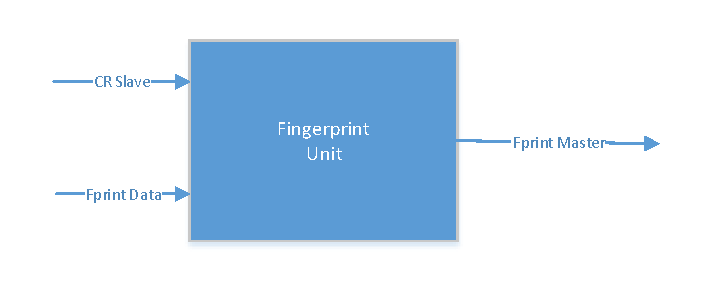
\includegraphics[scale=0.8]{Figures/fprint_icon}
\caption{Fingerprint unit ports.}
\label{f:fprint_icon}
\end{figure}

\begin{figure}[ht]
\centering
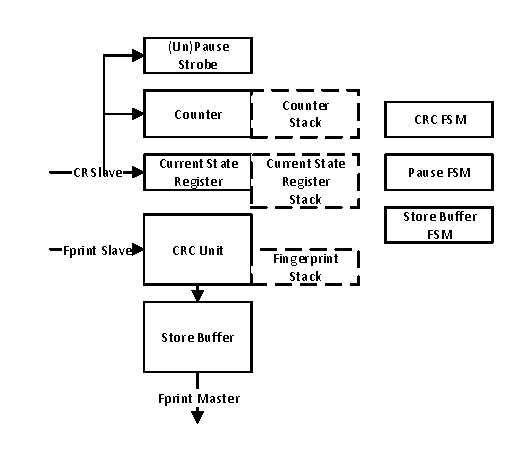
\includegraphics[width=10cm]{Figures/fprint_sch}
\caption{Schematic of the fingerprint unit components.}
\label{f:fprint_sch}
\end{figure}


\subsubsection{CRC Implementation}
The CRC implementation is shown in Figure \ref{f:crc}. A detailed explanation of how the CRC circuit is derived can be found in \cite{Hamed:12}. The circuit has been further modified to allow a \emph{variable} input data width. The implementation hinges on the RTLA multiplexers. For a $W$ bit circuit there will be $RTLA_i$ multiplexers indexed $1 < i < W$.
For an $M$ bit fingerprint, it is possible to shift the values in the RTLA to the right such that only the upper part of the circuit is used. This is useful for future implementations when load and store instructions will be used. For load instructions, only the address will be fingerprinted. By ensuring that the upper bits of the input $A_i$ are the address bits from the bus, it is possible to keep the block from being overly padded with zeros. In Figure \ref{f:rtla}, (a) shows the original RTLA while (b) and (c) show the updated RTLA capable of updating the fingerprint of either the address or the address and data inputs depending on whether or not the instruction is a store or a load. 

\begin{figure}[ht]
\centering
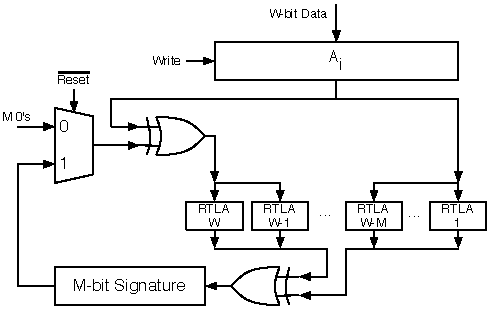
\includegraphics[width=10cm]{Figures/crc}
\caption{Implementation of CRC algorithm.}
\label{f:crc}
\end{figure}

\begin{figure}[ht]
\centering
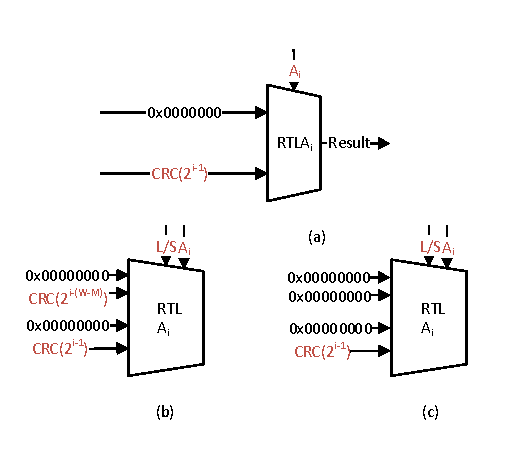
\includegraphics[scale=1]{Figures/rtla}
\caption[RTLA modification]{\emph{RTLA modification:} (a) original RTLA. (b) The RTLA for the upper portion of the input. When a load instruction is being fingerprinted the lower RTLA values are shifted right. (c) The lower portion of the input is completely deactivated during load instructions.}
\label{f:rtla}
\end{figure}

\subsubsection{Preventing state corruption during pause}
As was already discussed in Chapter \ref{Chapter2}, it is not possible to pause fingerprinting without causing at least one erroneous store instruction. Therefore each state register is doubled in order to store the \emph{previous} value to the latest calculation. It is the previous value that is pushed onto the stack to be restored when a task is unpaused. Furthermore, it is important to ensure that there are mechanisms to catch whether the erroneous store \emph{completes} a fingerprinting block. In the current implementation, the store buffer holds onto fingerprints until either a pause strobe or any other event occurs that changes state. The fingerprint is discarded if a pause strobe is the next event. Otherwise it is sent to the comparator. 

\subsection{Comparator}
The comparator collects fingerprints from all the cores in a system and compares them. The current implementation of the comparator is limited to 16 cores and two-way comparison. Ideas previously discussed in the interface sections as well as Chapter \ref{Chapter2} will receive less thorough treatment. Figure \ref{f:comp_sch} shows the comparator schematic with all the main components. Figure \ref{f:comp_fsm} shows the comparator FSM. The implementation of the comparator is quite involved and somewhat counter-intuitive and the best way to understand how it behaves as a whole is to directly examine the Verilog code. A summary of each state will be given. Three new data structures must first be introduced: the \emph{Fprint Trigger} register and the \emph{Checkin and Checkout} registers, and the \emph{Head and Tail Pointers}.

\begin{figure}[ht]
\centering
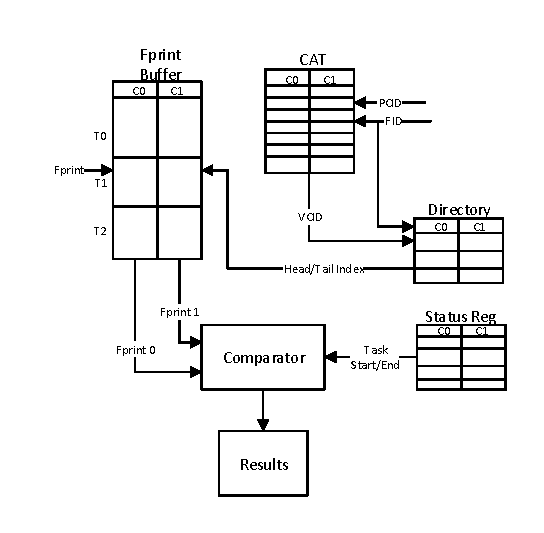
\includegraphics[scale=1.5]{Figures/compsch}
\caption[Comparator schematic]{\emph{Comparator schematic:} The FID, PCID and fingerprint arrive from the fingerprint unit. The FID and PCID are embedded in the address offset. The CAT is used to determine the VCID. The directory uses the VCID to locate the head pointer for the given FID. The comparator communicates with all the data structures but these signals have been omitted for clarity.}
\label{f:comp_sch}
\end{figure}
The \emph{Fprint Trigger} register keeps track of when the first new fingerprint arrives for a task since the last fingerprint was compared. This register is necessary because the arrival of a fingerprint is not in itself an event that should trigger comparison. Only once new fingerprints are available from both cores should a comparison be done. Also, in the case where a comparison cannot immediately be serviced, for instance if fingerprints arrive from several different tasks at once, the comparator can easily keep track of what is left to be done. The \emph{Checkin and Checkout} registers are simply registers that maintain a record of whether a task has started or ended on either of the virtual cores. The \emph{head and tail} registers keep track of the position of each task within the fingerprint queue. Remember that each task has its own start and end pointers that define a subset of the total fingerprint memory for a circular queue.

\begin{enumerate}
\item{\emph{Init:} The comparator is in an initial wait stage until an event occurs. Either a task has completed or a fingerprint has arrived.}
\item{\emph{Set Task:} The FID that caused the event is retrieved.}
\item{\emph{Load Pointer:} The tail pointer of the associated FID is loaded}
\item{\emph{Load Fprint:} The fingerprints are retrieved from the fingerprint buffer using the tail pointer.}
\item{\emph{Check Task Status:} If the checkin is activated for the given FID, then the task has completed(State 6). Otherwise proceed to State 7 to compare fingerprints.}
\item{\emph{Task Complete:} If the two head pointers match, then the same number of fingerprints arrived for both cores and the task was successful. Otherwise there was a problem (but no comparison took place because the comparator waits for new fingerprints from \emph{both} cores.}
\item{\emph{Compare Fprints:} If the fingerprints match then the tail pointer should be incremented (State  10). Otherwise a mismatch is detected.}
\item{\emph{Mismatch Detected:} An error has occurred.}
\item{\emph{Task Verified:} The task has been verified.}
\item{\emph{Increment Tail Pointer:} After a fingerprint comparison occurs, it is necessary to increment the tail pointer to proceed to the next comparison.}
\item{\emph{Check if Done:} This state checks whether for some reason several fingerprints were waiting to be compared, in which case the next comparison occurs. Otherwise the Fprint Trigger bit for the current FID is reset.}
\item{\emph{Reset Fprint Trigger:} Reset the Fprint Trigger bit for the current FID.}
\item{\emph{Reset Head and Tail:} The head and tail pointers for the given task should be reset when an error occurs.}
\item{\emph{Write Status Reg:} The status register should be updated and an interrupt will be sent to the Monitor. Further updates to status register can be made up until the monitor responds to the interrupt.}
\end{enumerate}




\begin{figure}[ht]
%\centering
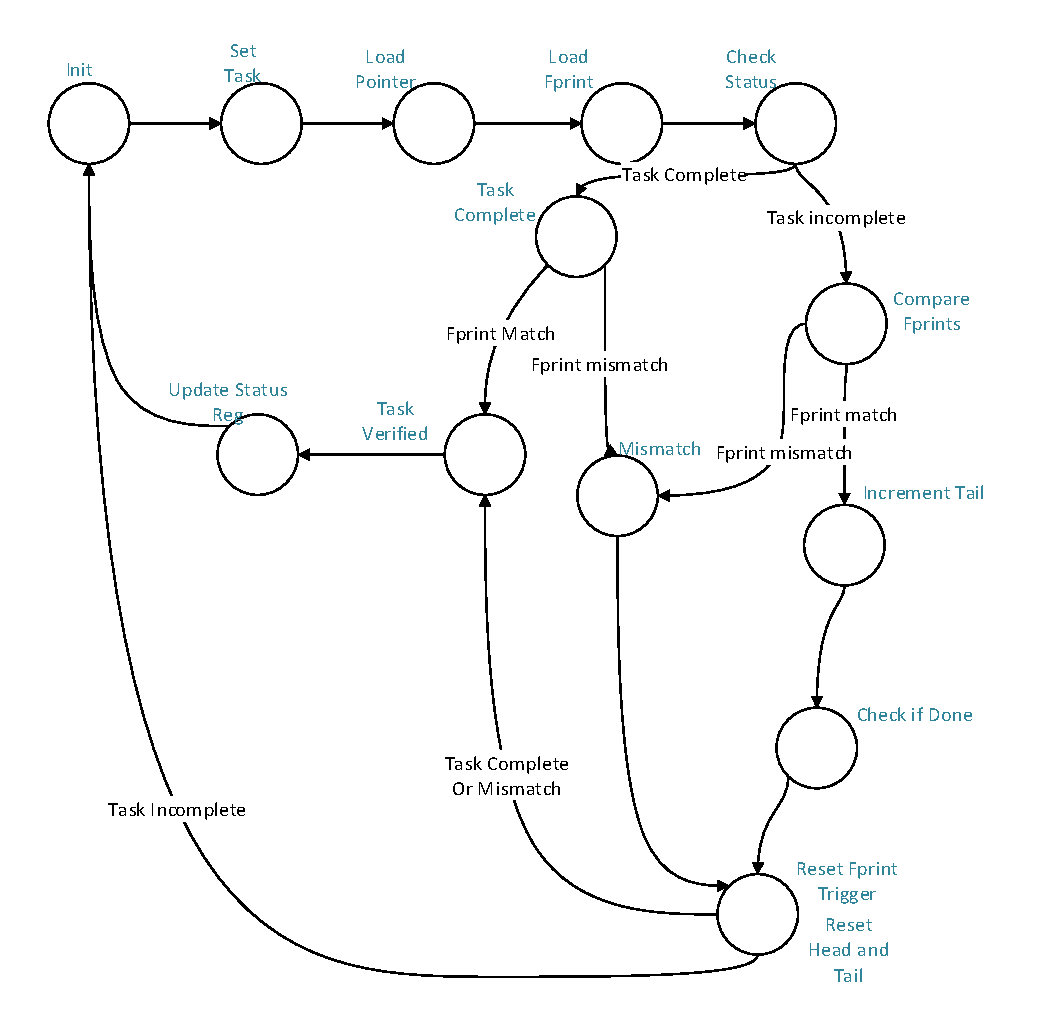
\includegraphics{Figures/comp_fsm}
\caption{Comparator FSM}
\label{f:comp_fsm}
\end{figure}



 
\chapter{Open Virtual Platform Model and Multicore Debugging} % Main chapter title

\label{Chapter4} % For referencing the chapter elsewhere, use \ref{Chapter1} 

\lhead{Chapter 4. \emph{Virtual Platform Model and Multicore Debugging}} % This is for the header on each page - perhaps a shortened title

\section{Virtual Platform Overview}
Several important and interrelated trends in embedded systems that are forcing designers to reconsider basic issues of design and verification methodologies. Firstly, there is the emergence of distributed real-time applications running on integrated multicore platforms. Secondly, there is the necessity of hardware software co-design: the platform and application development must often take place in parallel. Thirdly, heterogeneous MPSoCs, systemswith different types of cores and hardware accelerators, provide a wide range of power and efficiency tradeoffs where the optimal mapping of application to resources must be aware of the platform resources. There is also the emerging area of reconfigurable computing where the hardware and software can adapt and reconfigure based on changing system state, thus adding an extra layer of flexibility and complexity to the picture of the heterogeneous platform.

The emergence of increasingly complex architectures makes testing and verification significantly more difficult. This is compounded by the need to be able to begin software verification prior to platform availability. Furthermore, the iterative design process can be more tightly executed when these stages are done in parallel. Often, many types of problems can be anticipated in early stages of design. It is easy to iamgine a situation where hardware is designed in isolation prior to software and problems are discovered during the early stages of software development that could easily be fixed by adjusting the hardware requirements. This cannot be done if they are developed in series since by that point the development of the hardware will be too far along to allow large structural changes. If they are designed in parallel, then optimal solutions that take into account both hardware and software adjustments can be considered and large trade-off decisions can be made with a fuller picture of the system in mind.

This has led to the development of increasing sophisticated and powerful platform simulation environments. Commercial products such as Imperas Multicore Development kit based off the Open Virtual Platform (OVP) standard as well as Mentor's Questa Multicore Simulator suggest that the debugging of distributed embedded software on virtual platforms is growing in popularity. 

With all that said, this project is much more modest in scope and may not have required platform virtualization if a team with more experience had tackled the software and hardware design in isolation. Being an inexperienced designer and having no background in formal testing or verification, it was very difficult to develop a comprehensive testing strategy for the hardware. This was very much an iterative learning process. The size of the project came to encompass both hardware and software. The possibility arose for bugs in the software or hardware in isolation, or due to a lack of understanding or foresight as to how the interface between hardware and software might behave. But there was no easy way to test the two halves of the problem in isolation, stimulating them with test vectors that approximated the other half. Quite a bit of progress was made over the first year, but quite a bit of time was also wasted. Confidence disappears and paranoia sets in when you are unsure if the current solution to the problem will work, even if executed perfectly. This lack of confidence can be a tremendous burden when strange behaviours are noticed in the system that can simultaneously arise from several bugs in the software and hardware as well as miscalculations in the initial conception. This is exacerbated by a lack of visibility into the system and no ability to isolate components and recreate system wide states. There's just a single ugly knot that needs untying and no obvious place to start loosening it.

\section{OVP Overview}

Platform virtualization with OVP provides several capabilities that have dramatically increased productivity when debugging new features since its development. The basic OVP workflow is shown in Figure \ref{f:ovp} Firstly, there is full system visibility. Breakpoints can be placed at any point in the code of any processor. Secondly, peripherals are treated as processor models. They are independent code threads activated by the simulator, meaning that they can also be debugged and breakpoints inserted in their functional model. Complex chains of events can be monitored automatically using scripts and full system visibility that are not possible when running on an FPGA. Full traces of all processors can be captured. Peripherals can be distilled to their most basic functional description while also presenting to the processors exact and identical control register interfaces. Code compiled using the Nios IDE given a QSYS generated platform specification runs with no modifications on the OVP platform derived from the same specifications. Functional verification of the hardware software interface can take place with much greater ease. Especially in the case where a bug arises out of an interaction between some software and hardware element, since in the virtual platform hardware is translated into software, it is much more easy to visualize, isolate, and remedy the problem.

\begin{figure}[h]
\centering
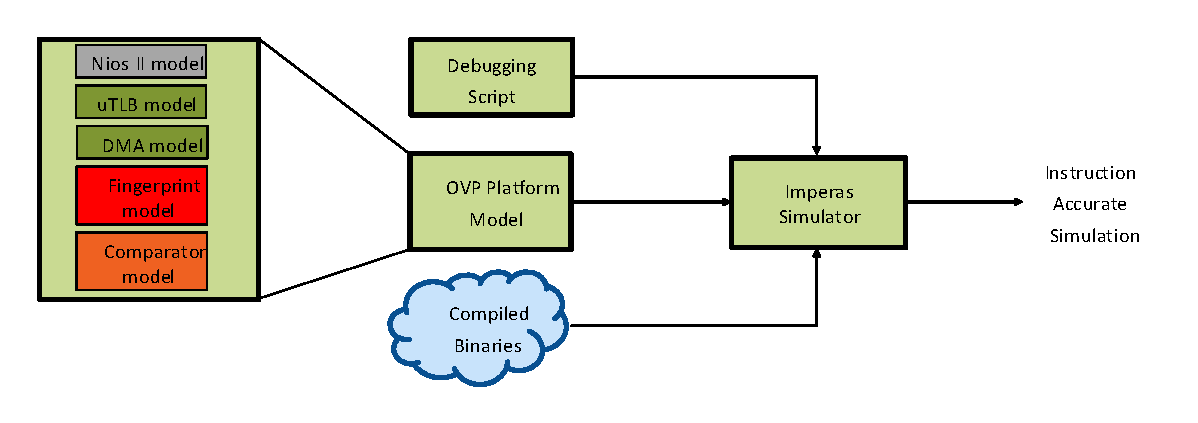
\includegraphics[scale=0.8]{Figures/ovp}
\caption{Platform virtualization workflow}
\label{f:ovp}
\end{figure}

\section{Processor Model}

The OVP processor model for the Nios II processor was co-developed with Altera and is fairly complete. Since the simulator is instruction accurate and does not take into account timing issues, the cache is omitted. Memory protection and memory management are available. One crucial aspect of the OVP system is that it is fully open source, allowing for modifications to the processor model to be made with relative ease. 

Fingerprinting involves a very strange type of peripheral that is concerned with all bus activity regardless of whether or not it is being addressed. Neither Quartus or OVP includes a built in mechanism for specifying a peripheral with this property. Therefore, it was note a trivial task to prepare the initial platform model that included a fingerprinting peripheral. 

The solution to the problem is ugly and is probably inefficient from a simulation speed perspective but it works and the technical details will now be discussed.

\subsection{Imperas Binary Intercept Technology}

In the OVP model, there are two types of behavioural descriptions: morph-time and run-time. The morph-time  API is used when creating a model description for the simulator to load the model. The run-time API is used to initiate behaviours while the simulator is running. Furthermore, there is a separate peripheral simulation engine (PSE). As it turns out, the processor simulation environment does not provide an easy way to do a seemingly simple thing. It is possible to add outgoing nets from a processor (although this is generally not done because the only outgoing signals from a processor should be the bus and buses have their own distinct model and port type). It is not possible to add to an instruction a command that stimulates one of these nets. 

Here is a more concrete example. The bus object in simulation is quite an abstraction and there is no way for a peripheral to see what is happening unless it is directly addressed. Therefore one solution is to add outgoing nets to the processor, and to modify the store instruction to stimulate those nets with information about the bus. The problem is that the code which defines the store instruction behaviour is considered morph-time by the simulator. Even if run-time APIs are included they will not be run after the simulation initializes. While it is possible to add nets to a processor, it is not possible for the processor to write values to those nets when executing store instructions. 

The Imperas Binary Intercept Technology (BIT) is a tool that allows additional run-time specifications to be added to a model as a separate shared library when the model is being loaded by the simulator. It is possible to use this tool to intercept and alter instructions as well as to monitor the system with complex chains of assertions. This is the API from which Imperas has developed their own prepackaged set of verification libraries (VAPs) and is therefore very powerful and able to reach deeply into the simulation environment.

The BIT provides two behaviours that allow the custom nets to convey information about writes. Firstly, it is possible to create a watchpoint over the entirety of memory for each core in the system. Whenever a write instruction is executed, this watchpoint is triggered. The callback of this watchpoint can then identify the processor that issues the instruction, as well as the address and data. It can then stimulate the nets associated with that processor such that they provide the information that a store has occurred as well as the address and data. These nets can then be directly connected to a fingerprinting peripheral. The BIT constructor and callback are shown in Listing \ref{l:vmi_callback}. Notice that the nets can carry 32 bit numbers, therefore three nets can carry all the information about a store instruction and that the run-time API (vmirt...) functions correctly.

\begin{lstlisting}[frame=single,language=C,label=l:vmi_callback,caption=VMI Memory watchpoint constructor and callback.]
//
// Constructor - install read and write callbacks on processor data domain
//
static VMIOS_CONSTRUCTOR_FN(constructor) {
    memDomainP domain   = vmirtGetProcessorPhysicalDataDomain(processor);
    Uns8       bits     = vmirtGetDomainAddressBits(domain);
    Addr       highAddr = (1ULL<<bits)) - 1;
    vmirtAddWriteCallback(domain, 0, 0, highAddr, writeCB, object);
}
static VMI_MEM_WATCH_FN(writeCB) {
    // we are interested only in writes made by processors (not artifacts of
    // simulation or memory accesses by other plugins, for example) so take
    // action only if processor is non null
    if(processor) {
        vmirtWriteNetPort(processor, vmirtGetNetPortHandle(processor, 
                "fprint_write_out_address"), address);
        vmirtWriteNetPort(processor, vmirtGetNetPortHandle(processor, 
                "fprint_write_out_data"), *((unsigned *)value));
        vmirtWriteNetPort(processor, vmirtGetNetPortHandle(processor, 
                "fprint_write_out"), 1);
    }
}
\end{lstlisting}

\section{Peripheral Models}
It was necessary to model the Altera provided DMA, mutex, as well as modify a prepackaged model of the Altera system timer. It was further necessary to model the comparator, the fingerprinting unit, the custom TLB, and the intercore IRQ bridge. The comparator and fingerprinting unit, including register sets, have been discussed already in some detail. This section will will give an overview of the DMA core and the TLB. The IRQ bridge is simply a bunch of register connected to the IRQ inputs of each core. Similarly the mutex is just a single register. All other functionality related to mutex behaviour is implemented in the sofware driver. Some simulation specific modifications will also be discussed.

\subsection{DMA}
A functional model of the DMA core was derived from the specification given in \cite{altera_ip_ug}. The timing characteristics of the DMA and any features related to packet size were omitted. The DMA peripheral therefore consists of one thread and one callback function that is triggered when the control register is written to by a processor. In line 4 of Listing \ref{l:dma}, the control register callback checks if the "GO" bit in the control register is written and if the length register has a non zero value (these functions should be self explanatory). If so, an event is triggered, causing the main DMA thread (line 21) to proceed past its wait condition. It should be fairly clear without any specific knowledge of the API that the main thread then updates its BUSY bit, performs the entire memory transaction in a single burst. Finally it updates all of its status bits. and notifies the processor with an interrupt if interrupts are enabled.

\begin{lstlisting}[frame=single,language=C,label=l:dma,caption=DMA model.]

PPM_REG_WRITE_CB(regWr) {
    *(Uns32*)user = data;
    if(DMACSP_ab8_data.control.bits.GO == 1 && DMACSP_ab8_data.length.value > 0){
        bhmTriggerEvent(start);
    }
}

static void dmaBurst(void) {   
    Uns32 len = DMACSP_ab8_data.length.value;
    char* buff = malloc(len);
    ppmReadAddressSpace (handles.MREAD,  DMACSP_ab8_data.readaddress.value, 
        len, buff);
    ppmWriteAddressSpace(handles.MWRITE, DMACSP_ab8_data.writeaddress.value, 
        len, buff);
    free(buff);
    DMACSP_ab8_data.length.value = 0;
    DMACSP_ab8_data.status.bits.LEN = 1;
}

static void channelThread(void *user)
{
    while(1) {
         bhmWaitEvent(start);
        
        //Start transaction
        DMACSP_ab8_data.status.bits.BUSY = 1;
         dmaBurst();
        DMACSP_ab8_data.status.bits.BUSY = 0;
        DMACSP_ab8_data.status.bits.DONE = 1;
        DMACSP_ab8_data.status.bits.REOP = 1;
        DMACSP_ab8_data.status.bits.WEOP = 1;
        if(DMACSP_ab8_data.control.bits.I_EN == 1){
            ppmWriteNet(handles.DMA_IRQ, 1);   
        }
    }
}
\end{lstlisting}

\subsection{TLB}
While the processor model comes equipped with an MMU, the translation process is completely transparent from the point of view of the intercept library and therefore there would be no easy way to integrate the TLB for fingerprinting purposes directly into the model. The same problem occurs with the actual HDL because the Nios core is encrypted. Keep in mind that for fingerprints to match, when main memory is used to store redundant state rather than dedicated scratchpads, the virtual address is required for fingerprint calculation.

The code for the TLB is a bit more cumbersome. It depends on a simulation object called a dynamic bridge that creates mappings from one address to another when a peripheral has both a master and slave port. An incoming address on the slave will continue on to the new translated address defined by the bridge. There is no thread or activity as with the DMA. There is no callback associated with the virtual address. There is no local memory object in the TLB associated with that address. The processor's fingerprinting nets are still activated by the intercept library. The TLB functions as follows:
\begin{itemize}
\item Wait until the TLB is enabled
\item Create a dynamic bridge for each translation entry in its table
\item Sort the table
\item Fill in the remainder of the address space with dynamic bridges that do not translate.
\end{itemize}

\section{Compensating for Simulation Artifacts}

The series of dynamic bridges breaks the intercept library to some extent. Simulation artifacts arise that cause fingerprints to stop matching. Both the physical and virtual address arrive at the fingerprinting unit, and sometimes several copies of them can arrive. Therefore, an interface between the TLB and fingerprinting unit must be added in order to allow the fingerprinting unit to know when translation is on and which addresses are being translated so that it ignores the physical addresses. Also, if the same data and address arrive twice in a row, it is assumed to be an artifact and is ignored. In the rare event where a program writes the same data to the same address on consecutive stores, the model simply falls a bit short in terms of its faithfulness to the physical platform. The model is very slow and running simulations in this fashion are not ideal for doing actual fault injection simulations. As a result, there is not much concern at the moment if an injected fault, once we begin developing OS services to replicate and restart threads, is masked on extremely rare events by this defective behaviour. 


\section{Case Study: Generated Code}
\label{s:matlabstudy}

\subsection{Fingerprinting a Simulink generated control loop}
Model based design is fundamental to automotive software engineering. An increasing proportion of the millions of lines of code that are currently used to run modern cars are computer generated \cite{mossinger2010software}. Furthermore, whether soft core or hard core, ISAs are established and compiler tool chains are mature and stable. One advantage of this architecture over single core hardening techniques is that no access or changes to existing core designs are required at the microarchitectural level. It is similarly advantageous to be able to leverage existing compiler and model-based code generation tools without requiring modifications. This second example demonstrates how fingerprinting can be used to monitor redundant executions of Simulink generated control code integrated into a simple RTOS template and compiled with \emph{gcc}.

Simulink Coder was used to extract transmission control logic from an example of an automotive drive train model \cite{sim_trans}. It would defeat the purpose and convenience of Coder to be forced to comb through and restructure the code to obey some style that is not natively supported. There are two things to note about the style of code: one that supports ease of fingerprinting and one that requires more attention. Firstly, the algorithm is a discrete FSM that will deterministically produce the same outputs given identical inputs. The tasks will match at the instruction level. The areas requiring more attention is the handling of global variables. Since the code will make hardwired references to global variables (i.e. the compiler will insert the absolute addresses into load and store instructions or calculate their position based on a global pointer register) it is necessary to ensure that separate duplicate copies are made for each core and that neither core is able to corrupt the original copy until fingerprinting is completed and the tasks are known to have been successful. 

Memory protection strategies is currently outside the scope of this work but the technology for implementing them is obviously well established. We assume that mechanisms are in place such that it is not physically possible for either plain core to write to the original data once a copy has been made. The final writeback must be done by reliable DMA initiated by a fault tolerant core (A core might be required to move the data out of the scratchpad to make room for another task or to provide a reference copy of data for rollback/reexecution purposes).

Once the global variables are copied into the scratchpads of the plain cores, memory translation is enabled to reroute references to global references away from main memory to the scratchpad. A full power MMU and OS virtualization services are not required. It is sufficient to ensure using linker options that the global variables are located in a contiguous block of data page aligned in accordance with the tag size of the uTLB and to annotate the global variables in the C code to be placed in the desired memory section. Meanwhile, the task stack must also be fit into the scratchpad and is accessed using its local physical address. As a further precaution, the global pointer register on each core are changed to match the GP register of whichever core the critical tasks were compiled for in case the compiler inserts GP relative address calculations. The context switch assembly code located in the BSP is then updated to include saving, resetting, and restoring the global pointer register so that any local interrupt handling code is not corrupted by a modified global pointer register should an interrupt occur during the critical task. 
 
\chapter{Experimental Results} % Main chapter title

\label{Chapter5} % For referencing the chapter elsewhere, use \ref{Chapter1} 


\lhead{Chapter 5. \emph{Experimental Results}} % This is for the header on each page - perhaps a shortened title


\section{Experimental Setup}

	Experiments evaluated the area and performance overhead of fingerprinting system compared with alternatives that utilize (a) software voting or (b) strict lockstep execution.
	Circuit size and complexity were evaluated by considering the resource utilization of each of the three systems when synthesized using Nios cores targeting an Altera Arria V FPGA development board.
	
	We first synthesized an implementation of the three-core architecture illustrated in Figure~\ref{f:arch}.
	One Nios core stands in for the fault tolerant core (FTC);
		we do not take steps to harden it.
	Note that safety-critical versions of the Nios and Microblaze cores are available for license~\cite{alteraniossc}\cite{xilinx_lockstep};
		these cores could act as a monitor with improved fault tolerance over a standard core.
	The architecture of the software voting system is the same as that used for fingerprinting;
		all logic supporting fingerprinting and fingerprint comparison is disabled, and redundancy checking is performed once at the end of the task, in software.
	We also synthesized a single core system to estimate the performance of a platform with a single lockstep pair as a baseline for comparison against fingerprinting and software voting.
	An actual lockstep system would likely have lower performance, as comparison logic of some sort is likely on the critical path.
	The development of a standalone lockstep system is beyond the scope of this work.
	
	First, we investigated the performance overhead of fingerprinting using benchmarks from the automotive suite from MiBench~\cite{guthaus2001mibench}.
	We modified each of basicmath, bitcount, qsort, and susan corners for execution on our fingerprinting system;
		the different benchmarks represent tasks of different lengths, input and output sizes, and store densities.
	Each benchmark repeatedly performed a calculation and we shortened the benchmarks by adjusting the number of times the main loop iterated.
	The size of the input data for qsort and susan were shortened to fit in the scratch-pad memory.
	Developing a comprehensive scratch-pad (or locked cache) allocation strategy and implementation that balances data size and algorithm complexity against fault containment is a potential subject for future investigation.
	
	The lockstep system may execute each benchmark directly;
		no manipulation to accommodate task duplication is needed.
	For each of fingerprinting and software voting, the task must first be duplicated on the pair of unreliable cores by the fault-tolerant monitor core.
	This is handled with a simple task graph transformation.
	In the case of fingerprinting, the task is replicated;
		no voting task is needed because fingerprinting and comparison hardware manage voting and report directly to the FTC.
	In the case of software voting, an additional voting task, dependent on each replicated task, is inserted, and performed by the FTC.

	Next, we performed a proof-of-concept evaluation of error detection latency under fingerprinting for each of the same four benchmarks.
	In order to demonstrate the error detection capabilities of fingerprinting we inject an error at the software level by corrupting, in software, a single value in the inputs to one of the two redundant tasks.
	When measuring error detection latency, we pessimistically assume that the effect of the faulty input propagates immediately into the execution stream (in reality it takes some time before the faulty input value is read, processed, and passed through the fingerprinting system).

	We do not attempt to perform an exhaustive fault injection campaign or to characterize the performance of the CRC algorithm or CRC based fingerprinting as an error detection mechanism; prior work has already addressed these issues.
	A table of 32 bit CRC polynomials and their associated hamming distances (i.e. minimum number of bits for which an error can go undetected) over various ranges of message length is given by Koopman in ~\cite{koopman200232}.
	Error detection latencies and probabilities with CRC-based fingerprinting was studied by Liu et al. in \cite{Meyer:13} through a simulation-based fault injection campaign of 1 and 2 bit data corruptions to a PowerPC register file.
	
	
\section{Results}
\label{s:results}

\subsection{Resource Utilization}

	We compare the cost in logic cells, registers and memory (in bits) of the main components of the fingerprinting system allocated to each unreliable core in Figure \ref{f:pie}(a).
	The Nios II figure includes a 1kB instruction cache and memory protection unit.
	Within a single core (we define the core as the CPU and any peripherals for which the CPU has its own copy), the fingerprint unit utilizes 16\% in combinationals, 14\% in registers, and less than 1\% in memory. We do not count the uTLB and DMA directly as overhead because they are peripherals that can be leveraged by other functions unrelated to reliability (and fingerprinting can technically be accomplished without them).
	%\bmtodo{Here's the place to say something about the simplicity of the Nios II core.  Can we make a comparison against a LEON3 core, too?  We should also state that the size of the logic doesn't change as the core changes, as the fingerprinting system is  entirely external to the core it is monitoring.}

\begin{figure}[tb]
\centering
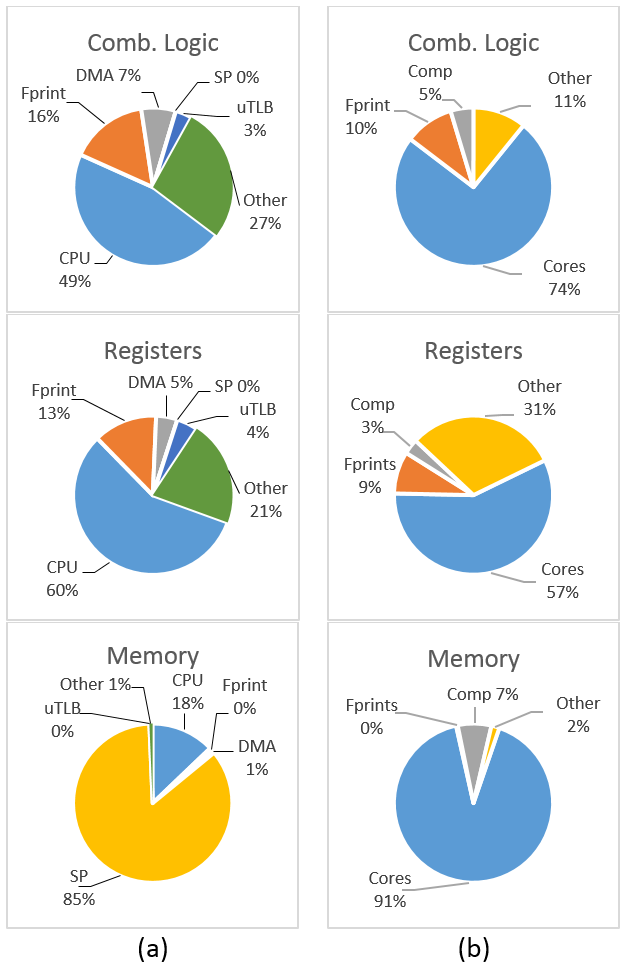
\includegraphics[scale=0.5]{figures/pie.png}
\caption[Fingerprinting FPGA resource allocation]{Fingerprinting FPGA overhead: (a) The local core and peripherals (b) The global system overhead}
\label{f:pie}
\end{figure}

	Figure \ref{f:pie}(b) shows the total cost of fingerprinting within a three core system where one core is assumed to be a reliable monitor and the two other cores are capable of fingerprinting.
	Therefore there are two fingerprinting units and a comparator added to the system.
	We note that the cost of the monitor core is probably too low because we have not implemented hardening or redundancy;
		this makes the relative cost of fingerprinting in this case pessimistic.
	The comparator represents only 6\% of combinationals, 4\% of registers and 7\% of onchip memory (excluding main memory).
	Note that the comparator is constant cost so long as the number of cores is less than 16, making this an upper limit cost;
		fingerprinting becomes more affordable the larger the number of cores that are supported.


\subsection{Single Task Replication and Detection Latency}

\begin{figure}[tb]
\centering
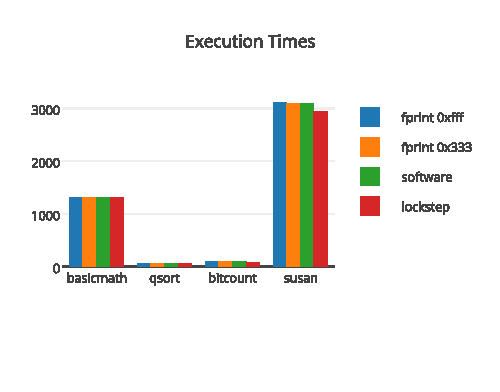
\includegraphics[scale=1.5]{Figures/execution_times}
\caption[Execution Time Results.]{\emph{Execution Time Results:} Four testbenches are executed on the three platforms. Fingerprinting is repeated with two different block sizes. There are no significant differences in execution time between any of the platforms.}
\label{f:extimes}
\end{figure}

	We compare the execution time of (a) lockstep DMR, (b) software voting, and (c) fingerprinting in Figure~\ref{f:extimes}.
	Fingerprinting is tested with two different block sizes.
	Execution time is measured from when the monitor first starts preparing the context of the other cores until it is notified that the task is completed, either by the comparator (under fingerprinting) or by the core themselves (under software voting).
	The performance of the fingerprinting and software checking platforms vary by less than 1\% for basicmath to 22\% for bitcount compared to the single core. The difference in execution time between fingerprinting and software checking is less than 1\% in all cases.
	The performance overhead associated with software checking and extra memory transactions (due to the fact that results must be copied from both cores) are not significant given the size of the data transfers compared to the lengths of the tasks.


\begin{figure}[tb]
\centering
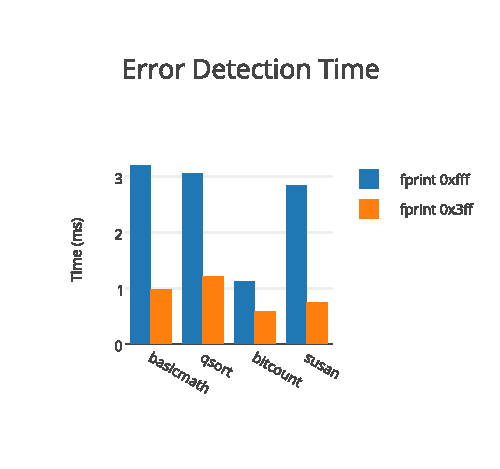
\includegraphics[scale=1.5]{Figures/error_detection_time}
\caption[Error detection latency]{The time it takes to detect an error with fingerprinting. Software voting cannot detect a fault until the task completes; lockstep DMR error detection latency varies based on implementation, but in some cases is no faster than fingerprinting.}
\label{f:dettimes}
\end{figure}

	In Figure~\ref{f:dettimes}, we report the error detection latency when one of the fingerprinted tasks is presented a faulty input.
	We observe that, as expected, the length of the fingerprinting block has an impact on detection latency.
	However, the placement of an error within a block and the density of store instructions will also have an effect.
	The bitcount testbench has such a different profile compared to the others because it uses bitwise operations as opposed to floating point which results in much more frequent pushing of data onto the stack. Furthermore, the erroneous input takes longer to affect the program execution.
		The detection latencies in Figure~\ref{f:dettimes} are significantly shorter than the execution times for a completed task; there is a potential to recover tens or even hundreds of extra milliseconds compared to software voting if a fault that occurs early in the execution of a task.
	
\subsection{Discussion}
	
	Consider again the Freescale Qorriva MPC577xK \cite{freescale2014qorivva} and Infineon Aurix 9x automotive ECUs \cite{infineon2014aurix} to place the resource utilization results in context. Firstly, a large amount of chip area on ECUs is devoted to interfacing with the external system. The Aurix chip, which is meant to be suited for several automotive applications that typically would have specialized ECUs, uses several serial bus controllers (e.g. I2C and Flex CAN), memory controllers, time management resources, interconnect logic, ADCs, and hardware security module. Secondly, the cores themselves are quite large and featured. The Qorriva Z7 cores have 16kB of instruction and data cache, 64 kB for data scratchpad, and FPUs. The lockstep functional safety core is also equipped with an FPU. Within this context, a fingerprint unit size of 30\% of the Nios core is quite reasonable. The Nios core we use has a 16kB scratchpad, 1kB instruction cache, no data cache or integer multiplication or division units and no MMU (future mixed criticality systems should expect to have full virtualization services to support hypervisors and more full-featured OS kernels such as Linux or Android). We argue that the comparison of fingerprint and CPU resource utilization on FPGA serves strictly as a rough measure demonstrating that the fingerprint unit is reasonably sized compared to the CPU and other peripherals that one might expect to find associated with each core. Furthermore, the size of comparator is reasonable taken against the size of the system when we consider that it supports up to 16 cores and that a realistic multicore ECU would be significantly larger than our prototype. Our platform excludes many peripherals and controllers such as IO interfaces, serial communication and memory controllers, ADC, PLL etc. 
	
	There are advantages to fingerprinting compared to core hardening techniques. While core hardening techniques exist that boast 10-15\% area overhead on custom CPU designs, they represent a a constant energy overhead whether the program running requires the higher reliability or not (i.e. they cannot be disabled). Furthermore, many core hardening techniques do not provide high enough coverage to support the most safety critical applications. Adoption of these techniques by manufacturers also poses a much greater risk since they require modifications to the CPU at the microarchitectural level. Fingerprinting is a non-invasive technique that can be integrated into a system without modifying the ISA or the CPU. Code can be written to be successfully fingerprinted without modifying the compiler toolchain or changing the code style from MISRA standards. We believe that fingerprinting is an ideal technique to be integrated into the automated design space exploration and code generation model-based design methodology because it provides several runtime tunable parameters and can be completely disabled.
	
	The main advantage of fingerprinting with respect to software checking and voting is the potential to greatly reduce detection latencies. Task level software checking suffers from large detection latency and increased memory transactions (although in the testbenches we examined these extra memory transactions were negligible). Single threaded software checking implemented by the compiler causes performance of the task to suffer and requires toolchain support (not tested in this paper but shown elsewhere). Multicore fault tolerant schedules require contingency plans in the case of failure. Fingerprinting reduces detection latencies which should eliminate the need for task grouping (which is done to reduce the overhead of voting and checking tasks) and can simplify the search for alternative schedules in the presence of multiple faults. Fingerprinting also has little to no impact on the performance of the task. Fingerprinting may cause very minor interference if it must use global buses to send information to the comparator. However these effects should be mitigated in a system with a deterministic (e.g. TDM) bus policy.	 
	
	
 
 
\chapter{Conclusions and Future Work} % Main chapter title

\label{Chapter6} % For referencing the chapter elsewhere, use \ref{Chapter1} 

\lhead{Chapter 6. \emph{Conclusions and Future Work}} % This is for the header on each page - perhaps a shortened title

\section{Impact	on	Society	and	the	environment}

	The environmental impact of this work is at best benign. The semiconductor industry faces a crisis because it relies on rare metals and does not take proper steps to ensure either their safe procurement or disposal. The conditions by which electronic devices are often recycled (when they are recycled) in large dumps and ludicrously unsafe working conditions in third world countries are well known. 
	
	I'm forced to wonder whether executives at TI and ST are mulling these problems over as they increasingly push their sensors and other embedded development products with the tag-line "Internet of Things". The IoT means more embedded microprocessors and sensors in increasingly cheap and disposable products, only exacerbating the unsustainable conditions that already exist. It may ultimately be a non-physical force that breaks Moore's Law. I don't believe the industry takes enough responsibility for these issues.
	
	With that said, I do believe that microelectronics represent a generally unacknowledged and misunderstood high form of art and craftsmanship. I believe that technology can empower people and have a significant positive impact on our quality of life. I also believe that this opportunity is largely squandered because technological innovation is being left largely to amoral corporate interests and should have more governmental oversight but that's another issue. I believe that transportation on this planet is set to undergo a massive reformulation as fossil fuels become increasingly problematic and alternative sources are only partially able to fill up the supply gap. Many people have already pointed out that the expansion of the middle class in India and China cannot realistically include a one-car-per-family lifestyle (see Figure \ref{f:jam}\cite{beij_traffic}). The amount of cars in the United States has already proven to be unscalable and the result of car culture on the urban landscape and social well-being to be generally bleak and negative. And the US is relatively sparsely populated compared to these emerging markets.
	
	The solution cannot be that smart cars will provide every citizen of this world with a private chauffeur. I hope that self-driving vehicles can be used to create a vastly superior system of public transportation than is currently feasible. I believe in making private ownership of vehicles illegal, or at least inverting the ratio of car lines to bus lanes in major cities. While this seems completely preposterous today, I think that a fleet of smart public transit operating on roads where human drivers are outlawed (but with heavy provisions made for pedestrian and bike traffic) will be the only way to efficiently move so many people around. (Think vast distributed network of automated Uber cars and buses that own their own traffic lanes).
	
	The domain of multicore embedded systems is in its infancy but it is crucial in realizing more sophisticated and smart robotics applications, from medical devices to automobiles to the next generation of addictive, trivial and mind-numbing commercial products. While the tools available to solve these problems are extensive, each problem is laboriously custom crafted and no generalized process exists. However, the last decade has seen much progress in defining the problem and possible paths forward. There is greater recognition that there are patterns and repetition in the individual solutions. I believe that the current state of technology is analogous to early single-core microprocessors when only assembly was available as a programming language. People eventually agreed upon less efficient but easier to program general and abstracted solutions to problems by introducing higher level programming languages. These abstractions increased the scope of a problem a single human could potentially solve with the given tool at the expense of some fine-grained efficiency losses. This work contributes a proposal to help efficiently ensure the feasibility of a multicore platform for mixed-criticality workloads.
	
\begin{figure}[h]
\centering
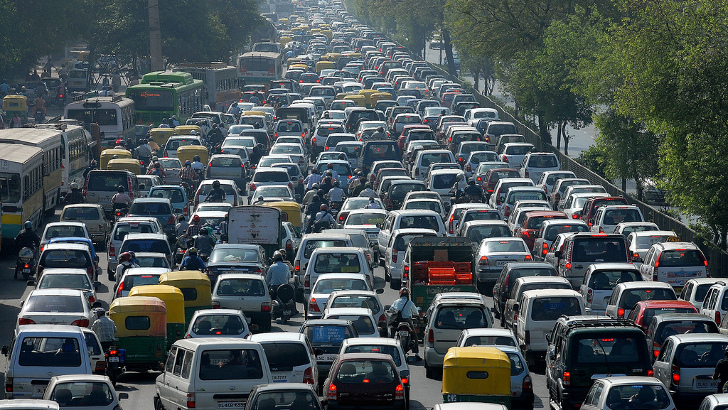
\includegraphics[width=10cm]{Figures/beijingtrafficjam.jpg}
\caption{A 12 day traffic jam occurred in Beijing in 2010.}
\label{f:jam}
\end{figure}
	
\section{Conclusions}
\label{s:conclusions}

	Heterogenous reliability architectures are a new and promising approach to deal with the variable safety requirements of mixed-criticality workloads. We have demonstrated that fingerprinting can be used to achieve dynamic core coupling and on-demand redundancy, which are themselves methods of significantly improving resource utilization when defining an application schedule and mapping to a platform. Fingerprinting represents a modest increase in logic for a multicore system while having the advantage over single core hardening techniques of being disabled (so as not to waste energy hardening non-critical tasks). Fingerprinting also provides shorter detection latencies compared to software checking on a fault tolerant core because it is not necessary to wait for the task to complete in order to verify it. By augmenting the fault tolerant core with a comparator module we remove the need for the FTC to take action until the result of a task is determined. The comparator is designed to function for up to 16 simultaneous tasks on up to 16 cores at constant cost for two way comparison and error detection. This method is not dependent on the bus topology without any special wiring. We have shown that is possible to implement fingerprinting on an FPGA platform without modifying or gaining access to the internal structure of the Nios II core. We have also demonstrated that it is possible to fingerprint a Simulink generated automotive shift logic controller requiring only modifications to the linker script and annotation of global variables in the header files. 
	
\section{Future Work}
	Several new questions arise for future research based on this prototype. Firstly, there is the possibility to recreate and extend the automated design space exploration process to include automated code generation for the platform. We can then explore the extent to which fingerprinting will affect the use of limited resources such as the data scratchpad. Secondly we can target the bus topology of our platform and replace the Altera Avalon bus with a time triggered statically scheduled bus policy. This will allow us to dramatically reduce interference in our system so that we can explore the possibility of fingerprint buffer overflow and how to mitigate it in dynamic applications with several nested tasks that all require fingerprinting.
	
	 

%----------------------------------------------------------------------------------------
%	THESIS CONTENT - APPENDICES
%----------------------------------------------------------------------------------------

\addtocontents{toc}{\vspace{2em}} % Add a gap in the Contents, for aesthetics

\appendix % Cue to tell LaTeX that the following 'chapters' are Appendices

% Include the appendices of the thesis as separate files from the Appendices folder
% Uncomment the lines as you write the Appendices

%% Appendix A

\chapter{User Configuration File} % Main appendix title

\label{A:ConfigFile} % For referencing this appendix elsewhere, use \ref{AppendixA}


The configuration file provided to the program must be able to express the basic flow as well as leave open the possibility of integrating extensions in the future. The syntax should be both easy to read for the user while also being easy to parse.

First, the functions must be specified. Each function must have a root name, a directory location as well as a constructor for global variables. The naming conventions for function names will follow the convention for Simulink generated code. The folder must contain the \texttt{ert\_main.c} file that provides variable declarations and initialization code.

The configuration file will be specified through examples. First, the function declarations:

\begin{lstlisting}[caption={Function configuration syntax},label=l:config-function,language=bash]
#periodic tasks, some are critical, all independent (no dataflow between tasks)


#function list must come first!!

#Comments start with #
# -c for critical task
# -T for task period in ms
# -E for event driven, runs when all the inputs are available
# -S for stacksize, if S is not present then assume profiler was used
# 	if profiler was used: should have a profile.log file in the function folders
<FUNCTIONLIST>
-rootdir /home/jonah/fingerprinting/automotive_control/CompiledC/for_loops
-name for_loop_100000_0    -subdir for_loop_100000_0           -T  30   -c  -Priority 2	
-name for_loop_50000_50000 -subdir for_loop_50000_50000		   -T  30       -Priority 1 -printRuntime -addPreamble preamble.txt
</FUNCTIONLIST>

#preamble -> in subdir folder, contains code to go before while loop in task, used for threadsafe newlib config, should not have extension .c or .h
#printRuntime adds diagnostic printf run time for the given task

<DATAFLOW>
</DATAFLOW>


<PLATFORM>
-usedefault
</PLATFORM>

<MAPPING>
for_loop_100000_0 cpu0 cpu1
for_loop_50000_50000 cpu0
</MAPPING>

#optional - skip stack profiling if included
<STACK_PROFILE>
for_loop_100000_0 80
for_loop_50000_50000 80
</STACK_PROFILE>


#optional - skip wcet profiling if included
<WCET_PROFILE>
for_loop_50000_50000 1600035
for_loop_100000_0 1600004 2400006
</WCET_PROFILE>
\end{lstlisting}


Whitespace is ignored except for line breaks. Each top level function must have a unique name and only be instantiated once.

%\input{Appendices/AppendixB}
%\input{Appendices/AppendixC}

\addtocontents{toc}{\vspace{2em}} % Add a gap in the Contents, for aesthetics

\backmatter

%----------------------------------------------------------------------------------------
%	BIBLIOGRAPHY
%----------------------------------------------------------------------------------------

\label{Bibliography}

\lhead{\emph{Bibliography}} % Change the page header to say "Bibliography"

\bibliographystyle{unsrtnat} % Use the "unsrtnat" BibTeX style for formatting the Bibliography

\bibliography{Bibliography} % The references (bibliography) information are stored in the file named "Bibliography.bib"

\end{document}  